% Options for packages loaded elsewhere
\PassOptionsToPackage{unicode}{hyperref}
\PassOptionsToPackage{hyphens}{url}
\PassOptionsToPackage{dvipsnames,svgnames,x11names}{xcolor}
%
\documentclass[
  letterpaper,
  DIV=11,
  numbers=noendperiod]{scrartcl}

\usepackage{amsmath,amssymb}
\usepackage{lmodern}
\usepackage{iftex}
\ifPDFTeX
  \usepackage[T1]{fontenc}
  \usepackage[utf8]{inputenc}
  \usepackage{textcomp} % provide euro and other symbols
\else % if luatex or xetex
  \usepackage{unicode-math}
  \defaultfontfeatures{Scale=MatchLowercase}
  \defaultfontfeatures[\rmfamily]{Ligatures=TeX,Scale=1}
  \setmainfont[]{Times New Roman}
  \setsansfont[]{Times New Roman}
\fi
% Use upquote if available, for straight quotes in verbatim environments
\IfFileExists{upquote.sty}{\usepackage{upquote}}{}
\IfFileExists{microtype.sty}{% use microtype if available
  \usepackage[]{microtype}
  \UseMicrotypeSet[protrusion]{basicmath} % disable protrusion for tt fonts
}{}
\usepackage{xcolor}
\setlength{\emergencystretch}{3em} % prevent overfull lines
\setcounter{secnumdepth}{5}
% Make \paragraph and \subparagraph free-standing
\ifx\paragraph\undefined\else
  \let\oldparagraph\paragraph
  \renewcommand{\paragraph}[1]{\oldparagraph{#1}\mbox{}}
\fi
\ifx\subparagraph\undefined\else
  \let\oldsubparagraph\subparagraph
  \renewcommand{\subparagraph}[1]{\oldsubparagraph{#1}\mbox{}}
\fi


\providecommand{\tightlist}{%
  \setlength{\itemsep}{0pt}\setlength{\parskip}{0pt}}\usepackage{longtable,booktabs,array}
\usepackage{calc} % for calculating minipage widths
% Correct order of tables after \paragraph or \subparagraph
\usepackage{etoolbox}
\makeatletter
\patchcmd\longtable{\par}{\if@noskipsec\mbox{}\fi\par}{}{}
\makeatother
% Allow footnotes in longtable head/foot
\IfFileExists{footnotehyper.sty}{\usepackage{footnotehyper}}{\usepackage{footnote}}
\makesavenoteenv{longtable}
\usepackage{graphicx}
\makeatletter
\def\maxwidth{\ifdim\Gin@nat@width>\linewidth\linewidth\else\Gin@nat@width\fi}
\def\maxheight{\ifdim\Gin@nat@height>\textheight\textheight\else\Gin@nat@height\fi}
\makeatother
% Scale images if necessary, so that they will not overflow the page
% margins by default, and it is still possible to overwrite the defaults
% using explicit options in \includegraphics[width, height, ...]{}
\setkeys{Gin}{width=\maxwidth,height=\maxheight,keepaspectratio}
% Set default figure placement to htbp
\makeatletter
\def\fps@figure{htbp}
\makeatother
\newlength{\cslhangindent}
\setlength{\cslhangindent}{1.5em}
\newlength{\csllabelwidth}
\setlength{\csllabelwidth}{3em}
\newlength{\cslentryspacingunit} % times entry-spacing
\setlength{\cslentryspacingunit}{\parskip}
\newenvironment{CSLReferences}[2] % #1 hanging-ident, #2 entry spacing
 {% don't indent paragraphs
  \setlength{\parindent}{0pt}
  % turn on hanging indent if param 1 is 1
  \ifodd #1
  \let\oldpar\par
  \def\par{\hangindent=\cslhangindent\oldpar}
  \fi
  % set entry spacing
  \setlength{\parskip}{#2\cslentryspacingunit}
 }%
 {}
\usepackage{calc}
\newcommand{\CSLBlock}[1]{#1\hfill\break}
\newcommand{\CSLLeftMargin}[1]{\parbox[t]{\csllabelwidth}{#1}}
\newcommand{\CSLRightInline}[1]{\parbox[t]{\linewidth - \csllabelwidth}{#1}\break}
\newcommand{\CSLIndent}[1]{\hspace{\cslhangindent}#1}

%\documentclass{article}

% todonotes package                          #####################

\usepackage[textsize=footnotesize]{todonotes}


%language                                    #####################

%\usepackage{times}
%\usepackage{t1enc}                               Trouble maker
%\usepackage[utf8x]{inputenc}
%\usepackage[polish]{babel}
%\usepackage{polski}


% math                                       #####################

%AMS
\usepackage{amsfonts}
\usepackage{amssymb}
\usepackage{amsthm}
\usepackage{amsmath}
\usepackage{mathtools}


% quote environment                        #######################  Unfortunately it destroys the font, only an issue in a mathmode

%\usepackage[T1]{fontenc} % Required for correct quotes with ""

%\renewenvironment{quote}
%{\list{}{\leftmargin=1em\rightmargin=1em}\item[]``}
%{''\endlist}



% page geometry                              #####################


\usepackage{geometry}
 \geometry{a4paper,left=35mm,top=20mm,}

\setlength{\parindent}{10pt}
\setlength{\parskip}{1pt}

\usepackage{float}
\restylefloat{figure}

% abbreviations                              #####################

\newcommand{\ra}{\rangle}
\newcommand{\la}{\langle}
\newcommand{\n}{\neg}
\newcommand{\et}{\wedge}
\newcommand{\jt}{\rightarrow}
\newcommand{\ko}[1]{\forall  #1\,}
\newcommand{\ro}{\leftrightarrow}
\newcommand{\exi}[1]{\exists\, {_{#1}}}
\newcommand{\pr}[1]{\mathsf{P}(#1)}
\newcommand{\cost}{\mathsf{cost}}
\newcommand{\benefit}{\mathsf{benefit}}
\newcommand{\ut}{\mathsf{ut}}

\newcommand{\dkl}{D_{\mathsf{KL}}} % trying to add the definition of \dkl

\newcommand{\odds}{\mathsf{Odds}}
\newcommand{\ind}{\mathsf{Ind}}
\newcommand{\nf}[2]{\nicefrac{#1\,}{#2}}
\newcommand{\R}[1]{\texttt{#1}}
\newcommand{\prr}[1]{\mbox{$\mathtt{P}_{prior}(#1)$}}
\newcommand{\prp}[1]{\mbox{$\mathtt{P}_{posterior}(#1)$}}

\newcommand{\s}[1]{\mbox{$\mathsf{#1}$}}


\newtheorem{q}{\color{blue}Question}
\newtheorem{lemma}{Lemma}


\newtheorem{theorem}{Theorem}
\newtheorem{definition}{Definition}        % trying to add the def. environment



% bibliography                                #####################

%\usepackage[authoryear]{natbib}  % solution to the  natbib compilation error

%\bibliographystyle{apalike}





\KOMAoption{captions}{tableheading}
\makeatletter
\makeatother
\makeatletter
\makeatother
\makeatletter
\@ifpackageloaded{caption}{}{\usepackage{caption}}
\AtBeginDocument{%
\ifdefined\contentsname
  \renewcommand*\contentsname{Table of contents}
\else
  \newcommand\contentsname{Table of contents}
\fi
\ifdefined\listfigurename
  \renewcommand*\listfigurename{List of Figures}
\else
  \newcommand\listfigurename{List of Figures}
\fi
\ifdefined\listtablename
  \renewcommand*\listtablename{List of Tables}
\else
  \newcommand\listtablename{List of Tables}
\fi
\ifdefined\figurename
  \renewcommand*\figurename{Figure}
\else
  \newcommand\figurename{Figure}
\fi
\ifdefined\tablename
  \renewcommand*\tablename{Table}
\else
  \newcommand\tablename{Table}
\fi
}
\@ifpackageloaded{float}{}{\usepackage{float}}
\floatstyle{ruled}
\@ifundefined{c@chapter}{\newfloat{codelisting}{h}{lop}}{\newfloat{codelisting}{h}{lop}[chapter]}
\floatname{codelisting}{Listing}
\newcommand*\listoflistings{\listof{codelisting}{List of Listings}}
\makeatother
\makeatletter
\@ifpackageloaded{caption}{}{\usepackage{caption}}
\@ifpackageloaded{subcaption}{}{\usepackage{subcaption}}
\makeatother
\makeatletter
\@ifpackageloaded{tcolorbox}{}{\usepackage[many]{tcolorbox}}
\makeatother
\makeatletter
\@ifundefined{shadecolor}{\definecolor{shadecolor}{rgb}{.97, .97, .97}}
\makeatother
\makeatletter
\makeatother
\ifLuaTeX
  \usepackage{selnolig}  % disable illegal ligatures
\fi
\IfFileExists{bookmark.sty}{\usepackage{bookmark}}{\usepackage{hyperref}}
\IfFileExists{xurl.sty}{\usepackage{xurl}}{} % add URL line breaks if available
\urlstyle{same} % disable monospaced font for URLs
\hypersetup{
  pdftitle={Second-order Probabilism: Expressive Power and Accuracy},
  pdfauthor={Rafal Urbaniak and Marcello Di Bello},
  colorlinks=true,
  linkcolor={blue},
  filecolor={Maroon},
  citecolor={Blue},
  urlcolor={Blue},
  pdfcreator={LaTeX via pandoc}}

\title{Second-order Probabilism: Expressive Power and Accuracy}
\author{Rafal Urbaniak and Marcello Di Bello}
\date{2024-04-15}

\begin{document}
\maketitle
\ifdefined\Shaded\renewenvironment{Shaded}{\begin{tcolorbox}[enhanced, boxrule=0pt, borderline west={3pt}{0pt}{shadecolor}, interior hidden, sharp corners, breakable, frame hidden]}{\end{tcolorbox}}\fi

\renewcommand*\contentsname{Table of contents}
{
\hypersetup{linkcolor=}
\setcounter{tocdepth}{3}
\tableofcontents
}
\vspace{2cm}

\noindent \textbf{DISCLAIMER:}
\textbf{This is a draft of work in progress, please do not cite or distribute without permission.}

\thispagestyle{empty}

\newpage

\begin{quote} \textbf{Abstract.}  \todo{need to write one when done}

\end{quote}

\hypertarget{introduction}{%
\section{Introduction}\label{introduction}}

\label{sec:introduction}

As rational agents, we form beliefs about a variety of propositions on
the basis of the evidence available to us. But believing a proposition
is not an all-or-nothing affair; it is a matter of degrees. We are
uncertain, to a greater or lesser extent, about the truth of many
propositions since the evidence we possess about them is often fallible.
To represent this uncertainty, it is natural to use a probability
measure that assigns to each proposition a value between 0 and 1 (also
called a degree of belief or credence). This approach---known as
\emph{precise probabilism}---models an agent's state of uncertainty (or
credal state) with a single probability measure: each proposition is
assigned one probability value (a sharp degree of belief). The problem
is that a sharp probability measure is not expressive enough to
distinguish between intuitively different states of uncertainty rational
agents may find themselves in (\S \ref{sec:precise-probabilism}). To
avoid this problem, a \emph{set} of probability measures, rather than a
single one, can be used to represent the uncertainty of a rational
agent. This approach is known as \emph{imprecise probabilism}. It
outperforms precise probabilism in some respects, but also runs into
problems of its own (\S \ref{sec:imprecise-probabilism}).

To make progress, this paper argues that the uncertainty of a rational
agent is to be represented neither by a single probability measure nor a
set of measures. Rather, it is to be represented by a higher-order
probability measure, more specifically, a probability distribution over
multiple probability measures. Call this view \emph{higher-order
probabilism}. We show that higher-order probabilism addresses all the
problems and philosophical puzzles that plague both precise and
imprecise probabilism (\S \ref{sec:higher-order} and
\S \ref{sec:proper-scores}).

Moreover, Bayesian probabilistic programming already provides a fairly
reliable implementation framework of this approach.

\todo{add structure description}

\todo{Think about including synergy}

\hypertarget{precise-probabilism}{%
\section{Precise probabilism}\label{precise-probabilism}}

\label{sec:precise-probabilism}

Precise probabilism (\textsf{PP}) holds that a rational agent's
uncertainty about a proposition is to be represented as a single,
precise probability measure. Bayesian updating regulates how the prior
probability measure should change in light of new evidence that the
agent learns. The updating can be iterated multiple times for multiple
pieces of evidence considered successively. This is an elegant and
simple theory with many powerful applications. Unfortunately,
representing our uncertainty about a proposition in terms of a single,
precise probability measure runs into a number of difficulties.

Precise probabilism fails to capture an important dimension of how our
fallible beliefs reflect the evidence we have (or have not) obtained. A
couple of stylized examples featuring coin tosses should make the point
clear.

\begin{quote}
\textbf{No evidence v. fair coin}
You are about to toss a coin, but have no evidence 
about its bias. You are completely ignorant. 
Compare this to the situation in which you know, 
based on overwhelming evidence, that the coin is fair. 
\end{quote}

\noindent On precise probabilism, both scenarios are represented by
assigning a probability of .5 to the outcome \emph{heads}. If you are
completely ignorant, the principle of insufficient evidence suggests
that you assign .5 to both outcomes. Similarly, if you know for sure the
coin is fair, assigning .5 seems the best way to quantify the
uncertainty about the outcome. The agent's evidence in the two scenarios
is quite different, but precise probabilities fail to capture this
difference.

\begin{quote}
\textbf{Learning from ignorance}
You toss a coin with unknown bias. You toss it 10 times and observe \emph{heads} 5 times. Suppose you toss it further and observe 50 \emph{heads} in 100 tosses. 
\end{quote}

\noindent Since the coin initially had unknown bias, you should
presumably assign a probability of .5 to both outcomes if you stick with
precise probabilism. After the 10 tosses, you again assess the
probability to be .5. You must have learned something, but whatever that
is, it is not modeled by precise probabilities. When you toss the coin
100 times and observe 50 heads, you learn something new as well. But
your precise probability assessment will again be .5.

These examples suggest that precise probabilism is not appropriately
responsive to evidence. Representing an agent's uncertainty by a precise
probability measure can fail to track what an agent has learned from new
evidence. Precise probabilism assigns the same probability in situations
in which one's evidence is quite different: when no evidence is
available about a coin's bias; when there is little evidence that the
coin is fair (say, after only 10 tosses); and when there is strong
evidence that the coin is fair (say, after 100 tosses). In fact,
analogous problems also arise for evidence that the coin is not fair.
Suppose the rational agent starts with a weak belief that the coin is .6
biased towards heads. They can strengthen that belief by tossing the
coin repeatedly and observing, say, 60 heads in 100 tosses. But this
improvement in their evidence is not mirrored in the .6 probability they
are supposed to assign to \emph{heads}.\footnote{Here is another problem
  for precise probabilism. Imagine a rational agent who does not know
  the bias of the coin. For precise probabilism, this state of
  uncertainty should be represented by a .5 probability assignment to
  the \emph{heads}. Next, the agent learns that the bias towards heads,
  whatever the bias is, has been slightly increased, say by .001. The
  addition of this new information is called \emph{sweetening} in the
  philosophical literature. This sweetening should now make the agent
  bet on heads: if the probability of \emph{heads} was initially .5, it
  must be ever so slightly above .5 after sweetening. But, intuitively,
  the new information should leave the agent equally undecided about
  betting on heads or tails. After sweetening, the agent still does not
  know much about the actual bias of the coin.}
\todo{add reference about sweetening}

These problems generalize beyond cases of coin tossing. It is one thing
not to know much about whether a proposition is true, for example,
whether an individual is guilty of a crime. It is another thing to have
strong evidence that favors a hypothesis and equally strong evidence
that favors its negation, for example, strong evidence favoring the
guilt hypothesis and equally strong evidence favoring the hypothesis of
innocence. Despite this difference, precise probabilism would reccomend
that a probability of .5 be assigned to both hypotheses in either case.
Here, too, precise probabilism fails to be appropriately responsive to
the evidence. In addition, evidence can accumulate in a way that does
not require changing our initial probability assignments. It could be
that, at first, one has stronger evidence for \(A\) than for \(B\). So
the probability assigned to \(A\) should be greater than the probability
assigned to \(B\). As more evidence accumulates, suppose the overall
evidence still favors \(A\) over \(B\) to the same degree. No change in
the probabilities is thus required. But something has changed about the
agent's state of uncertainty towards \(A\) and \(B\): the quantity of
evidence on which the agent can make their assessment that \(A\) is more
probable than \(B\) is larger. And yet, this change is not reflected in
the precise probabilities assigned to these propositions.

\hypertarget{imprecise-probabilism}{%
\section{Imprecise probabilism}\label{imprecise-probabilism}}

\label{sec:imprecise-probabilism}

What if we give up the assumption that probability assignments should be
precise? Imprecise probabilism (\textsf{IP}) holds that a rational
agent's credal stance towards a hypothesis is to be represented by a
\emph{set of probability measures}, typically called a representor
\(\mathbb{P}\), rather than a single measure \(\mathsf{P}\). The
representor should include all and only those probability measures which
are compatible with the evidence (more on this point later).\footnote{For
  the development of imprecise probabilism, see Keynes (1921); Levi
  (1974); Gärdenfors \& Sahlin (1982); Kaplan (1968); Joyce (2005);
  Fraassen (2006); Sturgeon (2008); Walley (1991). Bradley (2019) is a
  good source of further references. Imprecise probabilism shares some
  similarities with what we might call \textbf{interval probabilism}
  (Kyburg, 1961; Kyburg Jr \& Teng, 2001). On interval probabilism,
  precise probabilities are replaced by intervals of probabilities. On
  imprecise probabilism, instead, precise probabilities are replaced by
  sets of probabilities. This makes imprecise probabilism more general,
  since the probabilities of a proposition in the representor set do not
  have to form a closed interval.} It is easy to see that modeling an
agent's credal state by sets of probability measure avoids some of the
shortcomings of precise probabilism. For instance, if an agent knows
that the coin is fair, their credal state would be represented by the
singleton set \(\{\mathsf{P}\}\), where \(\mathsf{P}\) is a probability
measure that assigns \(.5\) to \emph{heads}. If, on the other hand, the
agent knows nothing about the coin's bias, their credal state would be
represented by the set of all probabilistic measures, since none of them
is excluded by the available evidence. Note that the set of probability
measures does not represent admissible options that the agent could
legitimately pick from. Rather, the agent's credal state is essentially
imprecise and should be represented by means of the entire set of
probability measures.

So far as good. But, just as precise probabilism fails to be
appropriately evidence-responsive in certain scenarios, imprecise
probabilism runs in similar difficulties in other scenarios.

\begin{quote}
\textbf{Even v. uneven bias:}
 You have two coins and you know, for sure, that the probability of getting heads is .4, if you toss one coin, and .6, if you toss the other coin. But you do not know which is which. You pick one of the two at random and toss it.  Contrast this with an uneven case. You have four coins and you know that three of them have bias $.4$ and one of them has bias $.6$. You pick a coin at random and plan to toss it. You should be three times more confident that the probability of getting heads is .4. rather than .6.
\end{quote}

\noindent The first situation can be easily represented by imprecise
probabilism. The representor would contain two probability measures, one
that assigns .4. and the other that assigns .6 to the hypothesis `this
coin lands heads'. But imprecise probabilism cannot represent the second
situation. Since the probability measures in the set are all compatible
with the agent's evidence, no probability measure can be assigned a
greater (higher-order) probability than any other.\footnote{Other
  scenarios can be constructed in which imprecise probabilism fails to
  capture distinctive intuitions about evidence and uncertainty; see,
  for example, (Rinard, 2013). Suppose you know of two urns,
  \textsf{GREEN} and \textsf{MYSTERY}. You are certain \textsf{GREEN}
  contains only green marbles, but have no information about
  \textsf{MYSTERY}. A marble will be drawn at random from each. You
  should be certain that the marble drawn from \textsf{GREEN} will be
  green (\(G\)), and you should be more confident about this than about
  the proposition that the marble from \textsf{MYSTERY} will be green
  (\(M\)). In line with how lack of information is to be represented on
  \textsf{IP}, for each \(r\in [0,1]\) your representor contains a
  \(\mathsf{P}\) with \(\pr{M}=r\). But then, it also contains one with
  \(\pr{M}=1\). This means that it is not the case that for any
  probability measure \(\mathsf{P}\) in your representor,
  \(\mathsf{P}(G) > \mathsf{P}(M)\), that is, it is not the case that RA
  is more confident of \(G\) than of \(M\). This is highly
  counter-intuitive.}

These examples show that imprecise probabilism is not expressive enough
to model the scenario of uneven bias. Defenders of imprecise probabilism
could concede this point but prefer their account for reasons of
simplicity. They could also point out that imprecise probabilism models
scenarios that precise probabilism cannot model, for example, a state of
complete lack of evidence. In this respect, imprecise probabilism
outperforms precise probabilism in expressive power, but also retains
theoretical simplicity. Unfortunately, it is questionable whether
imprecise probabilism actually outperforms precise probabilism \emph{all
things considered}. As we will now seee, imprecise probabilism suffers
from a number of shortcomings that do not affect precise probabilism.

The first problem has not received extensive discussion in the
literature, but it is fundamental. Recall that, for imprecise
probabilism, an agent's state of uncertainty is represented by those
probability measures that are \emph{compatible} with the agent's
evidence. The question is, how should the notion of compatibility be
understood here? Perhaps we can think of compatibility as the fact that
the agent's evidence is consistent with the probability measure in
question. But mere consistency wouldn't get the agent very far in
excluding probability measures, as too many probability measures are
strictly speaking still consistent with most observations and data.
Admittedly, there will be clear-cut cases: if you see the outcome of a
coin toss to be heads, you reject the measure with \(\mathsf{P}(H)=0\),
and similarly for tails. Another class of cases might arise while
randomly drawing objects from a finite set where the true frequencies or
objective chances are already known, because the finite set has been
inspected. But such clear-cut cases aside, what else? In the end,
evidence will often be consistent with a probability measure.\footnote{Probability
  measures can be inconsistent with evidential constraints that agents
  believe to be true. Mathematically, non-trivial evidential constraints
  are easy to model (Bradley, 2012). They can take the form, for
  example, of the \emph{evidence of chances} \(\{ \mathsf{P}(X) = x\}\)
  or \(\mathsf{P}(X) \in [x,y]\), or \emph{structural constraints} such
  as ``\(X\) and \(Y\) are independent'' or ``\(X\) is more likely than
  \(Y\).'' These constraints are something that an agent can come to
  accept outright, but only if offered such information by an expert
  whom the agent completely defers to. But, besides these idealized
  cases, it is unclear how an agent could come to accept such structural
  constraints upon observation. There will usually be some degree of
  uncertainty about the acceptability of these constraints.}

A second, well-known problem for imprecise probabilism is belief
inertia. Precise probabilism offers an elegant model of learning from
evidence: Bayesian updating. Imprecise probabilism, at least
\emph{prima facie}, offers an equally elegant model of learning from
evidence, richer and more nuanced. It is a natural extension of the
classical Bayesian approach that uses precise probabilities. When faced
with new evidence \(E\) between time \(t_0\) and \(t_1\), the
representor set should be updated point-wise, running the standard
Bayesian updating on each probability measure in the representor:
\begin{align*} \label{eq:updateRepresentor}
\mathbb{P}_{t_1} = \{\mathsf{P}_{t_1}\vert \exists\, {\mathsf{P}_{t_0} \!\in  \mathbb{P}_{t_0}}\,\, \forall\, {H}\,\, \left[\mathsf{P}_{t_1}(H)=\mathsf{P}_{t_0}(H \vert E)\right] \}.
\end{align*}

\noindent The hope is that, if we start with a range of probabilities
that is not extremely wide, point-wise learning will behave
appropriately. For instance, if we start with a prior probability of
\emph{heads} equal to .4 or .6, then those measures should be updated to
something closer to \(.5\) once we learn that a given coin has already
been tossed ten times with the observed number of heads equal 5 (call
this evidence \(E\)). This would mean that if the initial range of
values was \([.4,.6]\) the posterior range of values should be narrower.

Unfortunately, this narrowing of the range of values becomes impossisble
whenever the starting point is complete lack of knowledge, as imprecise
probabilism runs into the problem of belief inertia (Levi, 1980). This
problem arises in situations in which no amount of evidence could lead
the agent to change their belief state, according to a given modeling
strategy. Consider a situation in which you start tossing a coin knowing
nothing about its bias. The range of possibilities is \([0,1]\). After a
few tosses, if you observed at least one tail and one heads, you can
exclude the measures assigning 0 or 1 to \emph{heads}. But what else
have you learned? If you are to update your representor set point-wise,
you will end up with the same representor set. For any sequence of
outcomes that you can obtain and any probability value in \([0, 1],\)
there will exist a probability measure (conditional on the oucomes) that
assigns that probability to \emph{heads}. Consequently, the edges of
your resulting interval will remain the same. In the end, it is not
clear how you are supposed to learn anything if you start from complete
ignorance.\footnote{Here's another example of inertia, coming from
  Rinard (2013). Either all the marbles in the urn are green (\(H_1\)),
  or exactly one tenth of the marbles are green (\(H_2\)). Suppose your
  initial credence about these two hypothesis is complete uncertainty
  with interval. Next, suppose you learn that a marble drawn at random
  from the urn is green (\(E\)). After using this evidence to condition
  each probability measure in your representor (which initially contains
  all possible probability measures over the relevant space) on this
  evidence, you end up with the same spread of values for \(H_1\) that
  you had before learning \(E\). This holds no matter how many marbles
  are sampled from the urn and found to be green. This is
  counterintuitive: if you continue drawing green marbles, even if you
  started with complete uncertainty, you should become more inclided
  towards the hypothesis that all marbles are green.}

Some downplay the problem of belief inertia. After all, if you started
with knowing truly nothing, then it is right to conclude that you will
never learn anything. Joyce (2010) writes:

\begin{quote}
You cannot learn anything in cases of pronounced ignorance simply
because a prerequisite for learning is to have prior views about how
potential data should alter your beliefs (p.~291)
\todo{add reference.Joyce, J. M. (2010). A Defence of Imprecise Credences in Inference and Decision
Making, *Philosophical Perspectives* 24, pp. 281–323.}
\end{quote}

\noindent The upshot is that vacuous priors should not be used and that
imprecise probabilism gives the right results when the priors are
non-vacuous. Another strategy is to say that, in a state of complete
ignorance, a special updating rule should be deployed.\footnote{Elkin
  (2017) suggests the rule of \emph{credal set replacement} that
  recommends that upon receiving evidence the agent should drop measures
  rendered implausible, and add all non-extreme plausible probability
  measures. This, however, is tricky. One needs a separate account of
  what makes a distribution plausible from a principled account of why
  one should use a separate special update rule when starting with
  complete ignorance.}

Finally, imprecise probabilism faces a third, deeper problem that does
not arise for precise probabilism. As it turns out, it is impossible to
define proper scoring rules for measuring the accuracy of a representor
set of probability measures. Workable \emph{scoring rules} exist for
measuring the accuracy of a single, precise probability measure, such as
the Brier score. These rules measure the distance between a rational
agent's probability measure (also called credence function) and the
actual value. A requirement of scoring rules is that they be
\emph{proper}: any rational agent will score their own probability
measure to be more accurate than any other. After all, if an agent
thought a different probability measure was more accurate, they should
switch to it. Proper scoring rules are then used to formulate
accuracy-based arguments for precise probabilism. These arguments show
(roughly) that, if your precise measure follows the axioms of
probability theory, no other measure is going to be more accurate than
yours whatever the facts are. Can the same be done for imprecise
probabilism? It cannot. Impossibility theorems demonstrate that no
proper scoring rules are available for representor sets. So, as many
have noted, the prospects for an accuracy-based argument for imprecise
probabilism look dim (Campbell-Moore, 2020; Mayo-Wilson \& Wheeler,
2016; Schoenfield, 2017; Seidenfeld, Schervish, \& Kadane, 2012).
Moreover, as shown by Schoenfield (2017), if an accuracy measure
satisfies certain plausible formal constraints, it will never strictly
recommend an imprecise stance, as for any imprecise stance there will be
a precise one with at least the same accuracy.

\hypertarget{higher-order-probabilism}{%
\section{Higher-order probabilism}\label{higher-order-probabilism}}

\label{sec:higher-order}

Let us take stock. Imprecise probabilism is more expressive than precise
probabilism. It can model the difference between a state in which there
is no evidence about a proposition (or its negation) and a state in
which the evidence for and against a proposition is in equipoise. But
imprecise probabilism has its own expressive limitations: it cannot
model the case of uneven bias. In addition, imprecise probabilism faces
difficulties that do not affect precise probabilism: the notion of
compatibility between a probability measure and the evidence is too
permissive; belief inertia trivializes Bayesian updating; and no proper
scoring rules exist for imprecise probabilism. In this section, we show
that higher-order probabilism overcomes the expressive limitations of
imprecise probabilism without falling prey to any such difficulties.

Proponents of imprecise probabilism already hinted to the need of
relying on higher order-probabilities. For instance, Bradley compares
the measures in a representor to committee members, each voting on a
particular issue, say the true chance or bias of a coin. As they acquire
more evidence, the committee members will often converge on a chance
hypothesis.

\begin{quote}
\dots the committee members are ``bunching up''. Whatever measure you
put over the set of probability functions---whatever ``second order
probability'' you use---the ``mass'' of this measure gets more and more
concentrated around the true chance hypothesis. (Bradley, 2012, p. 157)
\end{quote}

\noindent But such bunching up cannot be modeled by imprecise
probabilism alone: a probability distribution over chance hypotheses is
needed.\footnote{In a similar vein, Joyce (2005), in a paper defending
  imprecise probabilism, explicates the notion of weight of evidence
  using a probability distribution over chance hypotheses. Oddily,
  representor sets play no central role in Joyce's account of the weight
  of evidence.} That one should use higher-order probabilities has also
been suggested by critics of imprecise probabilism. For example, Carr
(2020) argues that sometimes evidence requires uncertainty about what
credences to have. Carr, however, does not articulate this suggestion
more fully, does not develop it formally, and does not explain how her
approach would fare against the difficulties affecting precise and
imprecise probabilism. We now set out to do precisely that.

The central idea of higher-order probabilism is this: a rational agent's
uncertainty is not single-dimensional and thus cannot be mapped onto a
one-dimensional scale like the real line. Uncertainty is best modeled by
the shape of a probability distribution over multiple probability
measures.\footnote{Bradley admits this much (Bradley, 2012, p. 90), and
  so does Konek (Konek, 2013, p. 59). For instance, Konek disagrees
  with: (1) \(X\) is more probable than \(Y\) just in case
  \(p(X)>p(Y)\), (2) \(D\) positively supports \(H\) if
  \(p_D(H)> p(H)\), or (3) \(A\) is preferable to \(B\) just in case the
  expected utility of \(A\) w.r.t. \(p\) is larger than that of \(B\).}
Stated more formally, a rational agent's state of uncertainty (or credal
stance) towards a proposition \(X\) is not represented by a single
probability value \(\mathsf{P}(X)\) between 0 and 1, but by a
probability (density) distribution \(f_{\mathsf{P}(X)}\), where the
first-order probability measure \(\mathsf{P}(X)\) is treated as a random
variable. Crucially, this representation is completely general. Unlike
the exaples used so far, the proposition \(X\) is not restricted to
chance hypotheses or the bias of a coin. The probability distribution
\(f_{\mathsf{P}(X)}\) assigns a second-order probability to each of the
first-order probabiilities \(\mathsf{P}(X)\).
\todo{check that wording is technically correct}

How should these second-order probabilities be understood? It is helpful
to think of higher-order probabilism as a generalization of imprecise
probabilism. Imprecisers already admit that some probability measures
are compatible and others incompatible with the agent's evidence at some
point. Compatibility is a coarse notion; it is an all-or-nothing affair.
But, as seen earlier, evidence can hardly exclude a probability measure
in a definitive manner except in clear-cut cases. Just as it is often a
matter of degrees whether evidence supports a proposition, the notion of
compatibility between evidence and probability measures can itself be a
matter of degrees. On this picture, the evidence justifies different
values of first-order probability to various degrees. So, second-order
probabilities express the extent to which the first-order probabilities
are supported by the evidence.

This higher-order approach at the technical level is by no means novel.
Bayesian probabilistic programming languages embrace the well-known idea
that parameters can be stacked and depend on each other (Bingham et al.,
2021). But, while the technical machinery has been around for a while,
it has not been deployed by philosophers to model a rational agent's
uncertainty or credal state. Because of its greater expressive power,
higher-order probabilism can represent uncertainty in a more
fine-grained manner, as illustrated in
Figure~\ref{fig-evidenceResponse}. In particular, the uneven coin
scenario in which the two biases of the coin are not equally
likely---which imprecise probabilism cannot model---can be easily
modeled within high-order probabilism by assigning different
probabilities to the two biases.

\begin{figure}[t]

{\centering 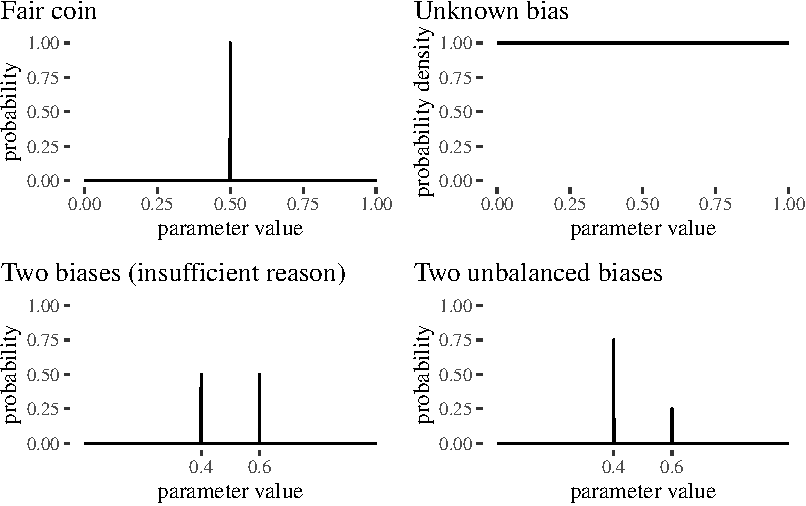
\includegraphics[width=0.8\textwidth,height=\textheight]{imp_philosophical_backup_files/figure-pdf/fig-evidenceResponse-1.pdf}

}

\caption{\label{fig-evidenceResponse}Examples of higher-order
distributions for a few scenarios problematic for both precise and
imprecise probabilism.}

\end{figure}

An agent's uncertainty could---perhaps, should---sometimes be
represented by a sigle probability value. Higher-order probabilism does
not prohibit that. For example, there may well be cases in which an
agent's uncertainty uncertainty is aptly represented by the
expectation.\footnote{The expectation is usually defined as
  \(\int_{0}^{1} x f(x) \, dx\). In the context of our approach here,
  \(x\) is the first-order probability of a given proposition, and \(f\)
  is the density representing the agent's uncertainty about \(x\).} But
this need not always be the case. If the probability distribution is not
sufficiently concentrated around a single value, a one-point summary
will fail to do justice to the nuances of the agent's credal
state.\footnote{This approach lines up with common practice in Bayesian
  statistics, where the primary role of uncertainty representation is
  assigned to the whole distribution. Summaries such as the mean, mode
  standard deviation, mean absolute deviation, or highest posterior
  density intervals are only succinct ways for representing the
  uncertainty of a given scenario.} For example, consider again the
scenario in which the agent knows that the bias of the coin is either .4
or .6 but the former is three times more likely. Representing the
agent's credal state with the expectation
\(\mathsf{P}(X) = .75 \times .4 + .25 \times .6 = .45\) would fail to
capture the agent's different epistemic attitudes towards the two
biases. The agent believes the two biases have different probabilities,
but is also certain the bias is \emph{not} .45.

Besides its greater expressive power in modelling uncertainty,
higher-order probabilism does not fall prey to belief inertia or the
impossibility of proper scoring rules. Consider a situation in which you
have no idea about the bias of a coin. You start with a uniform density
over \([0,1]\) as your prior. Observing any non-zero number of heads
will exclude 0 and observing any non-zero number of tails will exclude 1
from the basis of the posterior. The posterior distribution will become
more centered as the observations come in. This result is a
straightforward application of Bayesian updating. Instead of plugging
sharp probability values into teh formula for Bayes's theorem , the
factors to be mutiplied in the theorem will be probability densities (or
ratios of densities as needed). Figure~\ref{fig-intertia2}
illustrates---starting with a uniform prior distribution---how the
posterior distribution changes after successive observations of heads,
heads again, and then tails.\footnote{Assuming independence and constant
  probability for all the observations, learning is modeled the Bayesian
  way. You start with some prior density \(p\) over the parameter
  values. If you start with complete lack of information, \(p\) should
  be uniform. Then, you observe the data \(D\) which is the number of
  successes \(s\) in a certain number of observations \(n\). For each
  particular possible value \(\theta\) of the parameter, the probability
  of \(D\) conditional on \(\theta\) follows the binomial distribution.
  The probability of \(D\) is obtained by integration. That is:
  \begin{align*}
  p(\theta \vert D) & = \frac{p(D\vert \theta)p(\theta)}{p(D)}\\
  & = \frac{\theta^s (1-\theta)^{(n - s)}p(\theta)}{\int (\theta')^s (1-\theta')^{(n - s)}p(\theta')\,\, d\theta'}.
  \end{align*}}

\begin{figure}

{\centering 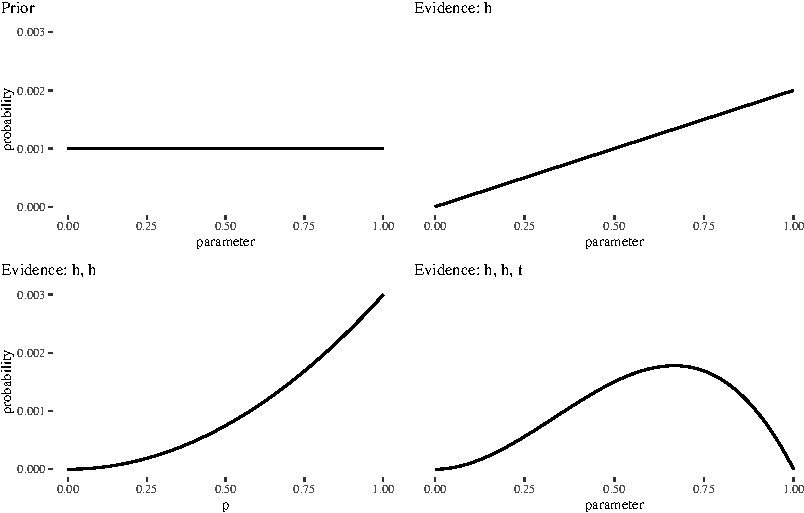
\includegraphics[width=0.8\textwidth,height=\textheight]{imp_philosophical_backup_files/figure-pdf/fig-intertia2-1.pdf}

}

\caption{\label{fig-intertia2}As observations of heads, heads and tails
come in, extreme parameter values drop out of the picture and the
posterior is shaped by the evidence.}

\end{figure}

The impossibility of proper scoring rules was another weakness of
imprecise probabilism. This is a significant shortcoming, especially
because proper scores do exist for precise probabilism. Fortunately, one
can show that there exist proper scoring rules for higher-order
probabilism. These rules can then be used to formulate accuracy-based
arguments. In addition, recall the point made by Schoenfield (2017): an
accuracy measure will not usually recommend an imprecise stance. This
argument fails against imprecise probabilism: there are cases in which
accuracy considerations recommend an imprecise stance (that is, a
multi-modal distribution) over a precise one. We will defend these
claims in the next section. It relies more heavily on a formal
apparatus, and it can be skipped without losing track of the main line
of the argument.

\hypertarget{proper-scoring-for-higher-order-probabilism}{%
\section{Proper scoring for higher-order
probabilism}\label{proper-scoring-for-higher-order-probabilism}}

\label{sec:proper-scores}

As already noted, one challenge for the imprecisers is providing a
proper scoring rule that would be a counterpart of, say, the Brier score
for the precise case. Imprecise probabilism cannot meet this challenge,
but we show that higher-order probabilism can.

The task is to define a score for comparing the accuracy of probability
distributions. As a first pass, we can help ourselves to existing work
on the accuracy of continuous probability distributions (Hersbach
(2000), Pettigrew (2012), Gneiting \& Raftery (2007)). The continuous
ranked probability score (CRPS) that assesses how well a probability
distribution aligns with a chance hypothesis that either puts all weight
on \(0\) or \(1\) can be of service here. The (CRPS) of a distribution
\(p\) with respect to a possible world \(w\) is defined as follows:
\begin{align*}
I(p,w) &= \int_{-\infty}^\infty \vert \mathsf{P}(x) - \mathbf{ 1 }(x\geq V(w))\vert ^2 \, dx
\end{align*} \noindent where \(\mathsf{P}\) is the cumulative
probability corresponding to the probability distribution \(p\), and
\begin{align*}
\mathbf{ 1 }(x \geq V(w)) & = \begin{cases} 1 & \text{ if } x \geq V(w)\\
0 & \text{ o$\,$/w. }
\end{cases}
\end{align*} \noindent   The CRPS score measures the distance relative
to an epistemically omniscient chance hypothesis, which either puts full
weight on \(0\), if a given proposition is false, or on \(1\),
otherwise.\footnote{The CRPS score is a particular case of the more
  general Cramer-Von-Mises measure of distance between densities,
  defined in terms of the area under the squared euclidean distances
  between the corresponding cumulative density functions: \begin{align*}
  \mathcal{C}(p,q) & = \int_{0}^{1} \vert P(x) - Q(x)\vert^2 \, dx
  \end{align*}} Measuring the distance between the cumulative
distributions helps capture the overall disparity between the predicted
and actual probabilities. The CRPS generalizes the Brier score as the
distance between the true value and the assigned probability to the case
of continuous probability distributions. We will start by reflecting on
this approach, but we will soon see that it runs into difficulties.

For computational ease, we will be using a grid approximation of the
densities, as in practice we are unable to work with infinite precision
anyway (note for instance that there are no readily computable solutions
to the integral used in the definition of CRPS, although it can
sometimes be evaluated in closed form) (Gneiting \& Raftery, 2007, p.
366) In parallel, we will be also using the Kullback-Leibler divergence:
\[
D_{\text{KL}}(p \,||\, q) = \sum_{x} p(x) \log\left(\frac{p(x)}{q(x)}\right)
\] \noindent which is a standard information-theoretic measure of
divergence of \(q\) from \(p\) from the perspective of
\(p\).\footnote{In the continuous case we'd need to use differential KL divergence.}

To fix ideas, consider a variation of a scenario by Schoenfield (2017).
A rational agent is invited to engage in a bet by an opponent who has
two coins. The behavior of the coins, instead of being described with
single point estimates, is described with parameters that reflect the
shape of the distribution of \(n\) tosses. One of these coins has a
normal distribution of \emph{Heads} centered at \(.3\), while the other
is centered at \(.5\). Both coins have a standard deviation of \(.05\).
The opponent randomly selects one of these coins and flips it. The
rational agent knows all the details of this set-up.

What credal state should the rational agent form in response? Consider
three options, but there could be more: first, a \emph{faithful bimodal}
distribution centered at \(.3\) and \(.5\); second, a \emph{unimodal}
distribution centered at \(.4\); third, a \emph{wide bimodal}
distribution centered at \(.2\) and \(.6\). The three options are
depicted in Figure~\ref{fig-emc}. All of them have expected values at .4
rounded to four digits.

\begin{figure}[H]

{\centering 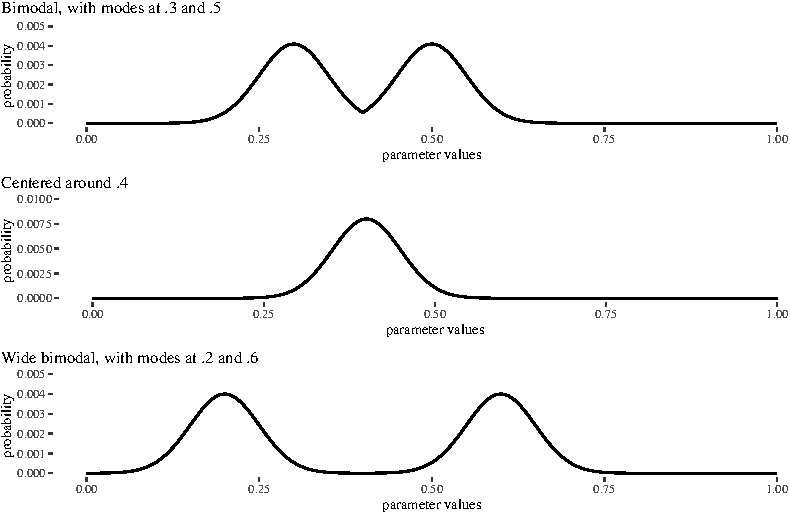
\includegraphics[width=1\textwidth,height=\textheight]{imp_philosophical_backup_files/figure-pdf/fig-emc-1.pdf}

}

\caption{\label{fig-emc}Three distributions in a vague EMS scenario. The
distributions are built from normal distributions with standard
deviation \(.5\), the bimodal ones are ``glued'' in the middle.}

\end{figure}

Denote these distributions as \(b, c, w\) correspondingly. Now consider
what happens if we think of expected inaccuracy of these distributions
with possible true outcomes, conceptualized as either heads (\(H\)) or
tails (\(T\)). Whatever our inaccuracy measure, we will have six
inaccuracy scores of the form
\(I(\mathsf{distribution}, \mathsf{outcome})\), where
\(\mathsf{outcome}\) is one of two omniscient distributions that give
all weight to either heads or tails. In the calculation of expected
values, these will need to be multiplied by the probability of \(H\) and
the probability of \(T\). However, none of these distributions assigns
such a probability, so to obtain such point values we in fact already
need to take expected values of the form
\(\mathbb{E}_{\mathsf{distribution}}(H) = \sum (x * \mathsf{distribution}(x))\),
where \(x\) are the values on the discretized grid (as in our example
these expectations are pretty much the same, we can simply take
\(\mathsf{distribution}(H)\) to be .4):

\[\mathbb{E}I_{binary}(p,q) = I(p,\mathsf{heads}) \mathbb{E}q(\mathsf{heads}) + I(p,\mathsf{tails}) \mathbb{E}q(\mathsf{tails}).\]

\noindent  Table \ref{tbl:comp1} displays the accuracy scores assigned
by CRPS assuming the true outcome is \emph{heads} (CRPS1) and assuming
the true outcome is \emph{tails} (CRPS0), and analogously for the KL
divergence. Then, we obtain the expected inaccuracies by averaging the
two scores by using the point probability of heads set to \(.4\). These
result in ExpCRPS and ExpKL respectively, note that since the
probability of heads is the same on all the distributions, those are
expected values from the perspective of each of the measures; changing
the perspective in this example doesn't change the expected inaccuracy.

\begin{table}[H]
\centering
\begin{tabular}{lrrrrrr}
\toprule
distribution & CRPS1 & CRPS0 & KLD1 & KLD0 & ExpCRPS & ExpKLD\\
\midrule
bimodal & 534.7305 & 334.9305 & 80.06971 & 33.90347 & 414.8505 & 52.36997\\
centered & 571.2192 & 371.4192 & 110.84220 & 53.13440 & 451.3392 & 76.21752\\
wide bimodal & 485.4052 & 285.6177 & 54.13433 & 19.50965 & 365.5340 & 33.35974\\
\bottomrule
\end{tabular}
\caption{CPRS and KLD inaccuracies of the three distributions to the TRUE and FALSE omniscient functions, with expected inaccuracies.}
\label{tbl:comp1}
\end{table}

As it turns out, the expected CRPS score recommends the wide bimodal
distribution as the most accurate (or least inaccurate). The KL
divergence from the omniscient measure makes the same
reccomendation.\footnote{This indicates that the choice of the
  evaluation metric is not the cause of the recommendation.} This is
counterintuitive because the faithful bimodal seems the one most
appropriately evidence-responsive. The unimodal distribution, while
centering on the expected value, gets the chances wrong, and the wide
bimodal has its guesses too close to the truth values and too far from
the known chances. But there is a further problem. While the wide
bimodal distribution expects itself to be the least inaccurate, the
other distributions also expect the wide bimodal to be the least
inaccurate. This indicates that in this setting the CRPS score and the
KL divergence are not proper scores, as they allow for cases of some
distributions recommending other distibutions as less accurate, whatever
the true state of the world turns out to be.

What are we to make of this result? Note that the three distributions
share the same expected value \(.4\). The latter is then used in the
calculations of the expected inaccuracies for both CRPS and KL. The
approach consists of (i) calculating two distances from the two extreme
omniscient measures and (ii) averaging by plugging in the expected
value. This approach, however, runs against the spirit of our
enterprise. If expected values are often not good representations of a
rational agent's uncertainty, it should not be surprising that relying
on them fails to deliver plausible expected accuracy scores. By reducing
each of the distributions' stance towards heads to a single point value
.4, we've effectively washed out key information. So the question is,
how can we adequately account for the complexity of a rational agent's
credal state in formulating a proper accuracy score?

Here is our proposal. Rather than measuring inaccuracy in relation to
``true states of the world'' conceptualized as two omniscient credences
that peak at either 0 or 1 and then averaging using expected values, we
should instead utilize a set of \(n\) potential true probability
hypotheses (ideally, going continuous, but we're working with a discrete
grid of \(n=1000\) possible coin baises in this paper). We then compute
all the inaccuracies with respect to each of these \(n\) values
represented by ``omniscient'' distributions (or true chance hypotheses)
and determine the expected inaccuracy scores using the entire
distributions rather than relying solely on their expected values.

\[\mathbb{E}I_{discretized}(p,q) = \sum  I(p,x) q(x),\]

\noindent where \(I(p,x)\) denotes the inaccuracy score of distribution
\(p\) from the omniscient distribution assigning all weight to \(x\),
for \(x\) belonging to the discretized grid.

For the three distributions under consideration, the accuracy scores
calculated using CRPS and KL divergence with respect to omniscient
distributions corresponding to various values of \(x\) are given by
Figure~\ref{fig-inaccuracies2}. The expected inaccuracies of the
distributions from their perspective are given by
\mbox{Table \ref{tbl:expected2}.} The results now match our common
sense: each distribution recommends itself. So, once we pay attention to
the whole range of possiblities, the CRPS score and KL divergence are
now proper scores.

\begin{figure}[H]

{\centering 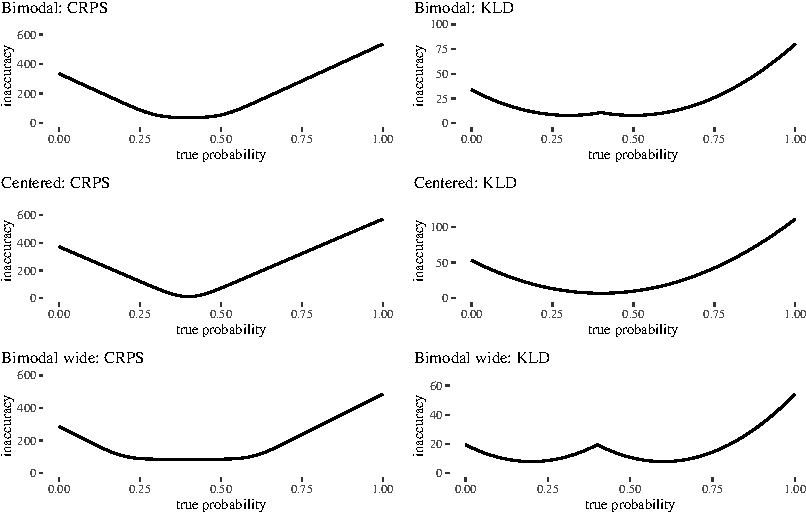
\includegraphics[width=1\textwidth,height=\textheight]{imp_philosophical_backup_files/figure-pdf/fig-inaccuracies2-1.pdf}

}

\caption{\label{fig-inaccuracies2}CLPSR and KL divergence based
inaccuracies vs (omniscient functions corresponding to) \(n\) true
probability hypotheses for the three distributions discussed in this
section.}

\end{figure}

\begin{table}[H]
\begin{tabular}{lrrrrrr}
& \multicolumn{3}{c}{CPRS} & \multicolumn{3}{c}{KLD} \\
\toprule
  & bimodal & centered & wide bimodal & bimodal & centered & wide bimodal\\
\midrule
bimodal & 64.670 & 78.145 & 88.380 & 8.577 & 10.655 & 11.336\\
centered & 41.657 & 28.181 & 85.911 & 9.239 & 7.690 & 15.627\\
wide bimodal & 137.699 & 171.719 & 113.989 & 11.541 & 19.231 & 8.689\\
\bottomrule
\end{tabular}
\caption{Expected inaccuracies of the three distributions from their own perspectives.
 Each row corresponds to a perspective.}
\label{tbl:expected2}
\end{table}

One important difference transpires between using CRPS and KLD. Notice
how for chance hypotheses between the actual peaks the inaccuracy
remains flat. This seems to be an artifice of choosing a squared
distance metric. If instead we go with a more principled,
information-theory-inspired KL divergence, inaccuracy in fact jumps a
bit for values in between the peaks for the bimodal distributions, which
seems intuitive and desirable. This seems to be a reason to prefer a
KL-based accuracy measure.

One question remains: how does the framework capture the idea that it is
the bimodal distribution that seems more adequate than the others? One
way to interpret that is by looking at inaccuracy concerning chance
hypotheses given by the testimonial evidence. In this case, these are
\(H_3\), where the true chance is \(0.3\), and \(H_5\), where the true
chance is \(0.5\). You can find the specific inaccuracies for them in
Table \ref{tbl:schoen}. To make sure that this favorable outcome isn't
due to not using pointed credences, we can redo the calculations using
the pointed version. In the pointed version, all the focus is on 0.4, or
the weight is evenly divided between 0.3 and 0.5, or between 0.2 and
0.6. As anticipated, when we consider inaccuracy, both of these setups
recommend the bimodal version (Table \ref{tbl:schoen2}).

\begin{table}[H]
\centering
\begin{tabular}{lrrrr}
 & \multicolumn{2}{c}{CRPS} & \multicolumn{2}{c}{KLD} \\
\toprule
&H3 & H5 & H3 & H5\\
\midrule
bimodal &55.475 & 55.378 & 7.935 & 7.935\\
centered &72.281 & 72.090 & 9.836 & 9.825\\
wide bimodal & 86.230 & 86.223 & 10.871 & 10.882\\
\bottomrule
\end{tabular}
\caption{CRPS and KLD inaccuracies of the three distributions with respect to the two hypotheses. On both inaccuracy measures the bimodal distribution dominates the other two.}
\label{tbl:schoen}
\end{table}

\begin{table}[H]
\centering
\begin{tabular}{lrrrr}
 & \multicolumn{2}{c}{CRPS} & \multicolumn{2}{c}{KLD} \\
\toprule
 &H3 & H5 & H3 & H5\\ \midrule
pointed bimodal &49.75 & 49.75 & 1.00 & 1.00\\
pointed centered &100.00 & 100.00 & 16.61 & 16.61\\
pointed wide bimodal & 99.75 & 99.75 & 16.61 & 16.61\\
\bottomrule
\end{tabular}
\caption{CRPS and KLD inacurracies of the three-pointed distributions with respect to the two hypotheses.}
\label{tbl:schoen2}
\end{table}

The discussion so far, while based on an example, may raise questions
about the strict propriety of the KLD as an inaccuracy measure. To
address this concern, a proof is provided in the appendix. In a
nutshell, the argument demonstrates that for a second-order discretized
probability mass \(p\) over a parameter space \([0,1]\), with the actual
probability denoted as \(\theta\), the Kullback-Leibler divergence of
\(p\) from the indicator distribution of \(\theta\) (which assigns 1 to
\(\theta\) and 0 to all other parameter values in the parameter space)
is expressed as \(\mathcal{I}_{\dkl}^2\).\footnote{The argument
  generalizes to parameter spaces that correspond to probabilities of
  multiple propositions which are Cartesian products of parameter spaces
  explicitly used in the argument in this section.} This serves as a
demonstration of the strict propriety of the inaccuracy measure: each
\(p\) anticipates itself to be the least inaccurate
distribution.\footnote{ The argument has four key moves:  

   
\begin{enumerate}
\item the inaccuracy of $p$ w.r.t. to parameter $\theta$ is just $- \log_2 p(\theta)$,
\item  the expected inaccuracy of $p$ from the perspective of $p$ is the entropy of $p$, $H(p)$,
\item  the inaccuracy of $q$ from the perspective of $p$ is the cross-entropy $H(p,q)$,
\item and it is an established result that cross-entropy is strictly larger than entropy as soon as $p\neq q$.
  \end{enumerate}
}

\hypertarget{evidence-aggregation}{%
\section{Evidence aggregation}\label{evidence-aggregation}}

The upshot so far is this. Higher-order probabilism outperforms both
precise and imprecise probabilism, at the descriptive as well as the
normative level. From a descriptive standpoint, higher-order probabilism
can easily model a variety of scenarios that cannot be adequately
modeled by the other versions of probabilism. From a normative
standpoint, accuracy maximization may sometimes recommend that a
rational agent represent their credal state with a distribution over
probability values rather than a precise probability
measure\todo{add ref to vFraasen in fn; perhaps extend the discussion a bit }
(more on this soon).\footnote{Having read van Fraasen's ``Laws and
  Symmetry'', you might also worry that going higher order somehow leads
  to a contradiction; we will address this concern later on.}
\todo{where do we show that accuracy recommends a distribution over probability measures? This bit seems missing.}
In this final section, we present a new challenge for imprecise
probabilism, and we show that higher-order probabilism can meet this
challenge.

Rational agents are often tasked with aggregating pieces of evidence and
assessing their value relative to a hypothesis. For two items of
evidence, \(E_a\) and \(E_B\), the posterior odds are obtained by
multiplying the likelihood ratio by the prior odds while filling in the
required probabilities:

\[
\frac{\pr{H \vert E_a \wedge E_b}}{\pr{\neg H \vert E_a \wedge E_b}} = \frac{\pr{E_a \wedge E_b \vert H}}{\pr{E_a \wedge E_b \vert \neg H}} \times \frac{\pr{H}}{\pr{\neg H}} 
\]

\noindent This is a straightforward application of Bayes's theorem in
odds form (often easier to use while carrying out calculations.) In the
simplest case, the pieces of information are independent lines of
evidence both relevant for hypothesis \(H\). Stated formally, \(E_a\)
and \(E_b\) are probabilistic independent conditional on hypothesis
\(H\). Think, for example, at two diagnostic tests performed by two
independent laboratories or two independent witnesses in a trial
testifying about the same issue. The posterior odds results from
multiplying the likelihood ratios associated with each piece of evidence
by the prior odds:

\[
\frac{\pr{H \vert E_a \wedge E_b}}{\pr{\neg H \vert E_a \wedge E_b}} = \frac{\pr{E_a \vert H}}{\pr{E_a \vert \neg H}}\times \frac{\pr{E_b \vert H}}{\pr{E_b \vert \neg H}} \times \frac{\pr{H}}{\pr{\neg H}} 
\]

\noindent In this simple case, precise probabilism seems well equipped
to handle evidence aggregation. (We will look at more complex scenarios
later.)

Unfortunately, precise probabilities are not always available. Even when
they are, they are not necessarily the best way to capture the
uncertainty of the situation. An example can illustrate this point.
Consider a murder case in which the police recover two items of trace
evidence, both against the defendant. First, hair found at the crime
scene matches the defendant's hair; call this evidence
\textsf{hair match}. Second, the fur of the defendant's dog matches the
fur found in a carpet wrapped around one of the bodies; call this
evidence \textsf{fur match}.\footnote{The hair evidence and the dog fur
  evidence are stylized after two items of evidence in the notorious
  1981 Wayne Williams case (Deadman, 1984b, 1984a).} The two matches
favor the hypothesis that the defendant (and the defendant's dog) must
be the source of the crime traces; call this hypothesis
\(\mathsf{source}\)). If the two matches are independent lines of
evidence (as they seem to be), their likelihood ratios can be
multiplied:\footnote{It is possible for \(A\) and \(B\) to be
  independent conditional on \(C\), but not conditional on \(\neg C\).
  Here, we require both independencies to hold.}

\[
\frac{{\pr{\s{dog} \wedge \s{hair}  \vert \s{source}}}}{{\pr{\s{dog} \wedge \s{hair} \vert \neg \s{source}}}} = \frac{{\pr{\s{dog} \vert \s{source}}}}{{\pr{\s{dog}  \vert \neg \s{source}}}} \times
 \frac{{\pr{\s{hair} \vert \s{source}}}}{{\pr{\s{hair} \vert \neg \s{source}}}}
\]

\noindent In assigning precise probabilities, the numerators can simply
be equated to one. If the defendant is a contributor, the laboratory
will declare a match for sure. To fill in the denominators, an expert
will provide the relevant random match probabilities, for example, by
counting of many matches are found in a representative sample of the
population. Suppose the matching hair type occurs 0.0253 times in a
reference database, and the matching dog fur type occurs 0.0256 times in
a reference database.\footnote{Probabilities have been slightly but not
  unrealistically modified to be closer to each other in order to make a
  conceptual point: the same first-order probabilities, even when they
  sound precise, may come with different degrees of second-order
  uncertainty (more on this soon). The original probabilities were 1/100
  for the dog fur, and 29/1148 for Wayne Williams' hair.} These
frequencies can be used to fill in the random match probabilities. So,
putting everything together: \begin{align*}
\frac{{\pr{\s{dog} \vert \s{source}}}}{{\pr{\s{dog}  \vert \neg \s{source}}}} \times
 \frac{{\pr{\s{hair} \vert \s{source}}}}{{\pr{\s{hair} \vert \neg \s{source}}}}
& =  \frac{1}{0.0252613} \times  \frac{1}{0.025641} = \frac{1}{\ensuremath{6.4772626\times 10^{-4}}}
\end{align*}

\noindent This is a large number. The combined match evidence is
strongly incriminating. It would be a huge coincidence if both matches
were due to mere chance.

\begin{figure}[H]

{\centering 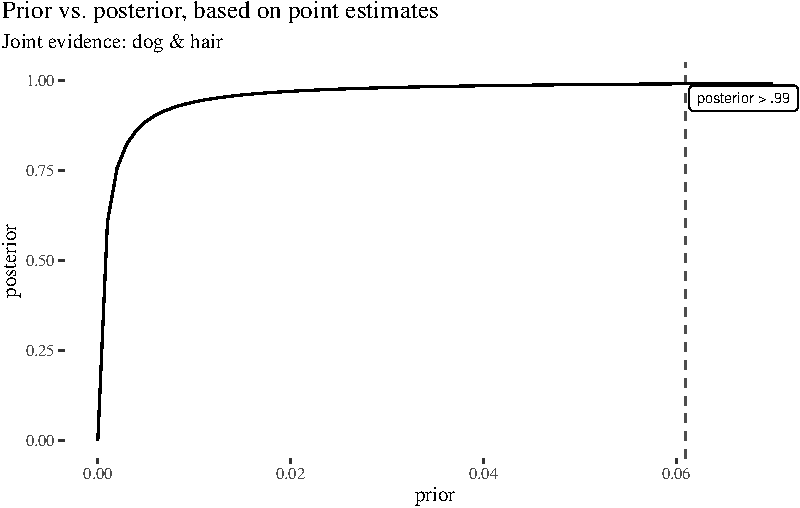
\includegraphics[width=0.6\textwidth,height=\textheight]{imp_philosophical_backup_files/figure-pdf/fig-impactOfPoint-1.pdf}

}

\caption{\label{fig-impactOfPoint}Impact of dog fur and human hair
evidence on the prior, point estimates.}

\end{figure}

So far so good. But precisely probabilism quickly runs into trouble
here. First, in order to find out the posterior odds, the likelihood
ratios must be multiplied by the prior odds
\(\frac{\pr{\s{source}}}{\pr{\neg \s{source}}}\). What precise value
should they take? This question is hard to answer definitively. To
circumvent this difficulty, Figure~\ref{fig-impactOfPoint} shows how the
items of match evidence, combined, change the probability of the source
hypothesis given a range of possible priors. This strategy---known as
\emph{sensitivity analysys}---shows that the posterior of .99 is reached
as soon as the prior is higher than 0.061.\footnote{These calculations
  assume that the probability of a match if the suspect and the
  suspect's dog are the sources is one.}

Sensitivity analysis moves away from precise probabilism. It gives up on
the prospect of assigning precise numbers to the prior probabilities.
The second problem with precise probabilism here is that the match
probabiltiies \(\pr{\s{dog} \vert \neg \s{source}}\) and
\(\pr{\s{fur} \vert \neg \s{source}}\) are also subejct to uncertainty.
They are assessed by looking at sample data. So why pick exactly the
numbers 0.0253 and 0.0256 for the match probabilities? Could they be
different?

Imprecise probabilism might seem well equipped to model the uncertainty
about match probabilities. But this is not so. In imprecise probabilism,
the probability measures in the representor set are those compatible
with the evidence, data or observations. Virtually any precise random
match probability is compatible with any sample data---with any number
of matches found in a reference database. Think by analogy to coin
tossing: even a coin that has a .99 bias toward tails could come up
heads on every toss. This series of outcomes is unlikely, but still
possible. Similarly, even a hair type that has a match probability
extremely small could be found several times in a sample population. So,
from the perspective of imprecise probabilism, it is not clear how to
proceed forward if one takes seriously the binary notion of
compatibility. Imprecise probabilism is so permissive that any match
probability will count as compatible with the data.

Another option is to identify reasonable ranges of probabilities. What
are the worst-case and best-case scenarios? Suppose the reasonable
ranges of the match probabilities are (.015,.037) (.002, .103), for hair
and fur evidence respectively.\footnote{These are 99\% credible
  intervals starting with uniform priors. A 99\% credible interval is
  the narrowest interval to which the expert thinks the true parameter
  belongs with probability .99. For a discussion of what credible
  intervals are, how they differ from confidence intervals, and why
  confidence intervals should not be used, see Kruschke (2015).} It is
enough to focus on what happens at the edges of the interval. Redoing
the calculations using the upper bounds of the two intervals, \(.037\)
and \(.103\), yields the following: \begin{align*}
\mathsf{P}(\s{dog}\wedge \s{hair} \vert \neg \s{source})   & =  .037 \times .103 =.003811.
\end{align*}

This number is around 5.88 times greater than the original estimate. Now
the prior probability of the source hypothesis needs to be higher than
0.274 for the posterior probability to be above .99
(Figure~\ref{fig-impactofcharitable}). The calculation for the lower
bounds, \(.015\) and \(.002\), yields the following: \begin{align*}
\mathsf{P}(\s{dog}\wedge \s{hair} \vert \neg \s{source})   & =  .015 \times .002 =.00003
\end{align*}

\noindent   This number is around 0.46 times lower than the original
estimate.

\begin{figure}[H]

{\centering 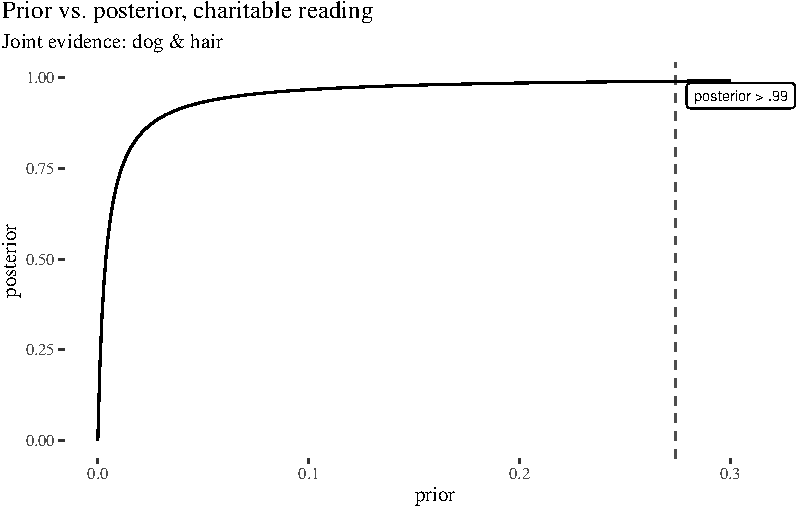
\includegraphics[width=0.6\textwidth,height=\textheight]{imp_philosophical_backup_files/figure-pdf/fig-impactofcharitable-1.pdf}

}

\caption{\label{fig-impactofcharitable}Impact of dog fur and human hair
evidence on the prior, charitable reading.}

\end{figure}

Using plausible ranges for the match probabilties leaves the impression
that any value in the interval is just as good as any other. But this
impression will often misrepresent the data. Figure~\ref{fig-densities}
(upper part) depicts the probability distribution of different match
probabilities given the sample data---the actual number of matches found
in the sample database. That is, 29 matches were found in a sample
database of human hair of size 1148, and 2 matches were found in a
sample database of dog fur of size 78. As expected, some random match
probabilities are more likely than others. And since the sizes of the
two databases are also different, the distribitions have different
spreads. The smaller the databse the greater the spread, the greater the
uncertainity about match probability. The trouble with imprecise
probabilims is that these nuanced information is entirely lost.

Figure~\ref{fig-densities} (lower part) depicts the probability
distribtion for the joint match probability associated with both items
of match evidence, hair and fur evidence.\\
Interestingly, the distribution for the joint evidence is not symmetric.
This means that the most likely value of the joint match probability
(and the bulk of the distribution, really) does not simply lie in the
middle between the edges. Therefore, only relying on the edges can lead
to overestimating or underestimating the probabilities at play.

\begin{figure}[H]

{\centering 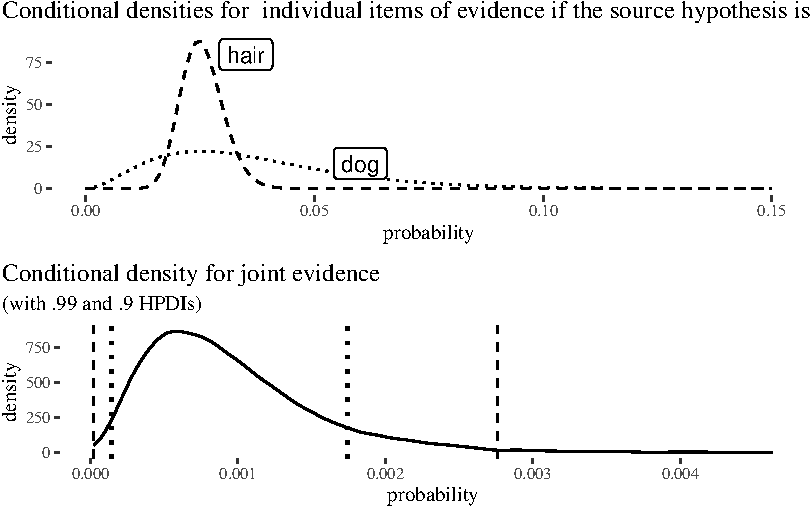
\includegraphics[width=0.8\textwidth,height=\textheight]{imp_philosophical_backup_files/figure-pdf/fig-densities-1.pdf}

}

\caption{\label{fig-densities}Beta densities for individual items of
evidence and the resulting joint density with .99 and .9 highest
posterior density intervals, assuming the sample sizes as discussed and
independence, with uniform priors.}

\end{figure}

\begin{figure}[H]

{\centering 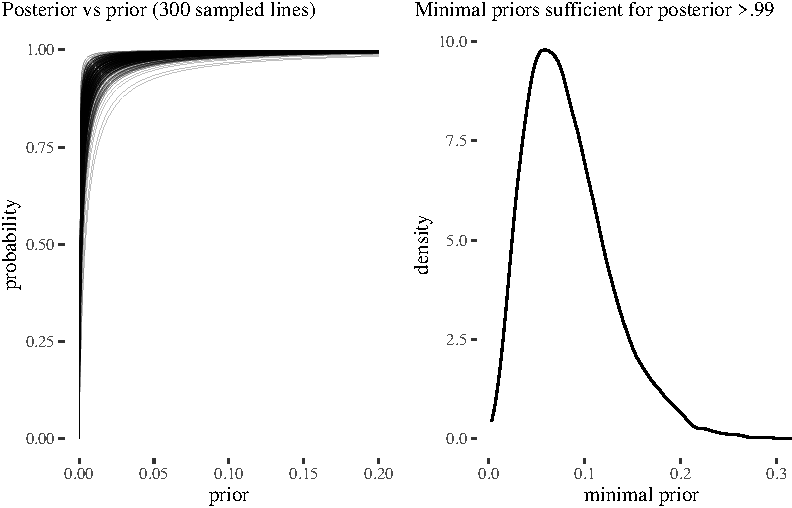
\includegraphics[width=0.8\textwidth,height=\textheight]{imp_philosophical_backup_files/figure-pdf/fig-lines-1.pdf}

}

\caption{\label{fig-lines}300 lines illustrating the uncertainty about
the dependence of the posterior on the prior given aleatory uncertainty
about the evidence, with the distribution of the minimal priors required
for the posterior to be above .99.}

\end{figure}

This, then, is the main claim illustrated in this section: higher-order
approach to evidence evaluation is more reliable and more honest about
the uncertainties involved. Whenever density estimates for the
probabilities of interest are available (and they should be available
for match evidence and many other items of scientific evidence if the
reliability of a given type of evidence has been properly studied),
those densities should be reported for assessing the strength of the
evidence. This approach avoids hiding actual aleatory uncertainties
under the carpet. It also allows for a balanced assessment of the
evidence, whereas using point estimates\\
or intervals may exaggerate or underestimate the value of the evidence.

Mathematically, we do not propose anything radically new---we just put
together some of the items from the standard Bayesian toolkit. The
novelty is rather in our arguing that that these tools are
under-appreciated in formal epistemology and in the legal scholarship
and should be properly used to incorporate second-order uncertainties in
evidence evaluation and incorporation.

\hypertarget{computational-and-representational-considerations}{%
\section{Computational and representational
considerations}\label{computational-and-representational-considerations}}

The higher-order framework we are advocating is not only applicable to
the evaluation of individual pieces of evidence. Complex bodies of
evidence and hypotheses---for example, those often represented by
Bayesian networks---can also be approached from this perspective. The
general strategy is this: (1) capture the uncertainties involving the
individual items of evidence in a modular fashion using the standard
tools for statistical inference. (2) Elicit other probabilities or
densities from experts\footnote{For expert elicitation of densities in a
  parametric fashion and the discussion of the improvement to which
  doing so instead of eliciting point values leads, see (O'Hagan et al.,
  2006).}, (3) put those together using a structure similar to that of a
Bayesian network, except allowing for uncertainties of various levels to
be put together --- a usual tool for such a representation is a
probabilistic program (Bingham et al., 2021), and (4) perform inference
evaluating the relevant probabilities or densities of interest.

If the reader is more used to thinking in terms of Bayesian networks, a
somewhat restrictive but fairly straightforward way to conceptualize a
large class of such programs is to imagine a probabilistic program as
stochastically generating Bayesian networks using our uncertainty about
the parameter values, update with the evidence, and propagate
uncertainty to approximate the marginal posterior for nodes of interest.

As an illustration, let us start with a simplified Bayesian network
developed by Fenton \& Neil (2018). The network is reproduced in Figure
\ref{fig-scbnplot} and represents the key items of evidence in the
infamous British case R. v. Clark (EWCA Crim 54, 2000).\footnote{Sally
  Clark's first son died in 1996 soon after birth, and her second son
  died in similar circumstances a few years later in 1998. At trial, the
  pediatrician Roy Meadow testified that the probability that a child
  from such a family would die of Sudden Infant Death Syndrome (SIDS)
  was 1 in 8,543. Meadow calculated that therefore the probability of
  both children dying of SIDS was approximately 1 in 73 million. Sally
  Clark was convicted of murdering her infant sons. The conviction was
  reversed on appeal. The case of appeal was based on new evidence:
  signs of a potentially lethal disease were found in one of the bodies.}

In a Bayesian network the arrows depict direct relationships of
influence between variables, and nodes---conditional on their
parents---are taken to be independent of their non-descendants.
\textsf{Amurder} and \textsf{Bmurder} are binary nodes corresponding to
whether Sally Clark's sons, call them A and B, were murdered. These
nodes influence whether signs of disease (\textsf{Adisease} and
\textsf{Bdisease}) and bruising (\textsf{Abruising} and
\textsf{Bbruising}) were present. Also, since A's death preceded in time
B's death, whether A was murdered casts some light on the probability
that B was also murdered.

The choice of the probabilities in the network is quite specific, and it
is not clear where such precise values come from. The standard response
invokes \emph{sensitivity analysis}: a range of plausible values is
tested. As already discussed, this approach ignores the shape of the
underlying distributions. Sensitivity analysis does not make any
difference between probability measures (or point estimates) in terms of
their plausibility, but some will be more plausible than others.
Moreover, if the sensitivity analysis is guided by extreme values, these
might play an undeservedly strong role. These concerns can be addressed,
at least in part, by recourse to higher-order probabilities. In a
precise Bayesian network, each node is associated with a probability
table determined by a finite list of numbers (precise probabilities).
But suppose that, instead of precise numbers, we have densities over
parameter values for the numbers in the probability tables.\footnote{The
  densities of interests can then be approximated by (1) sampling
  parameter values from the specified distributions, (2) plugging them
  into the construction of the BN, and (3) evaluating the probability of
  interest in that precise BN. The list of the probabilities thus
  obtained will approximate the density of interest. In what follows we
  will work with sample sizes of 10k.} An example for the Sally Clark
case is represented in Figure~\ref{fig-scwithhop}.

\begin{figure}[H]

{\centering 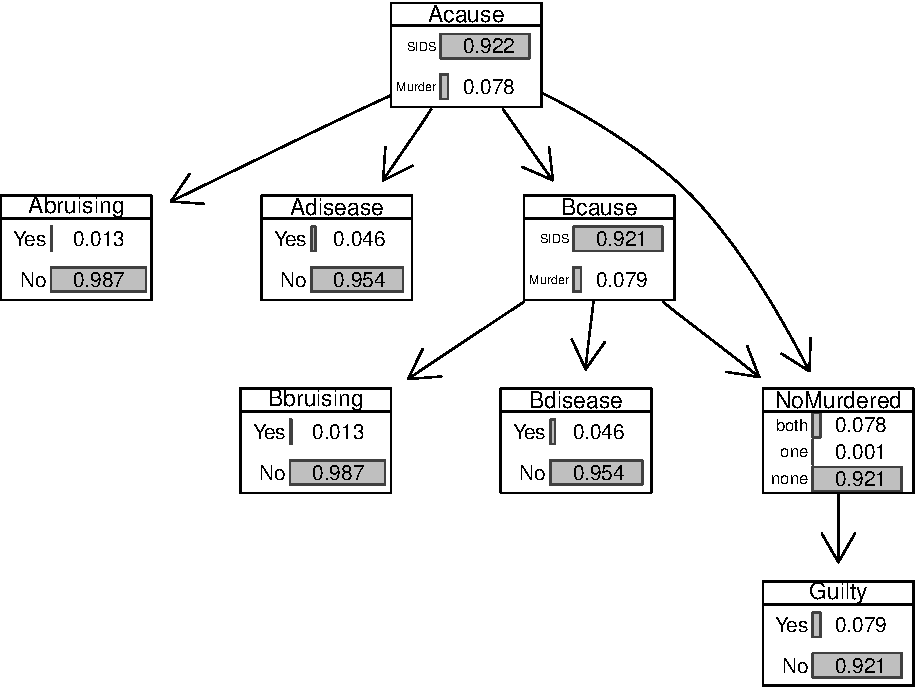
\includegraphics[width=0.8\textwidth,height=\textheight]{imp_philosophical_backup_files/figure-pdf/fig-scbnplot-1.pdf}

}

\caption{\label{fig-scbnplot}Bayesian network for the Sally Clark case,
with marginal prior probabilities.}

\end{figure}

\begin{figure}[h]

{\centering 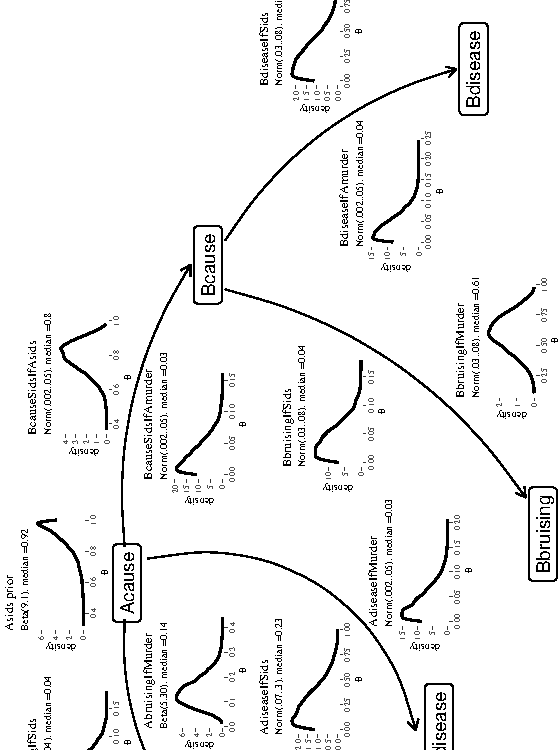
\includegraphics[width=1.25\textwidth,height=2.3\textheight]{imp_philosophical_backup_files/figure-pdf/fig-scwithhop-1.pdf}

}

\caption{\label{fig-scwithhop}An illustration of a probabilistic program
for the Sally Clark case.}

\end{figure}

\todo{N: I am still searching for a good fix of that plot}

Using the probabilistic program, we can investigate the impact of
different items of evidence on Sally Clark's probability of guilt
(Figure~\ref{fig-scwithhop}). The starting point is the prior density
for the \s{Guilt} node (first graph). Next, the network is updated with
evidence showing signs of bruising on both children (second graph).
Next, the assumption that both children lack signs of potentially lethal
disease is added (third graph). Finally, we consider the state of the
evidence at the time of the appellate case: signs of bruising existed on
both children, but signs of lethal disease were discovered only on the
first child. Interestingly, in the strongest scenario against Sally
Clark (third graph), the median of the posterior distribution is above
.95, but the uncertainty around that median is still too wide to warrant
a conviction.\footnote{The lower limit of the 89\% Highest Posterior
  Density Intervals (HPDI) is at .83.} This underscores the fact that
relying on point estimates can lead to overconfidence. Paying attention
to the higher-order uncertainty about the first-order probability can
make a difference to trial decisions.

\todo{nl: This plot is not referenced anywhere, should it be visible?}

\begin{figure}[H]

{\centering 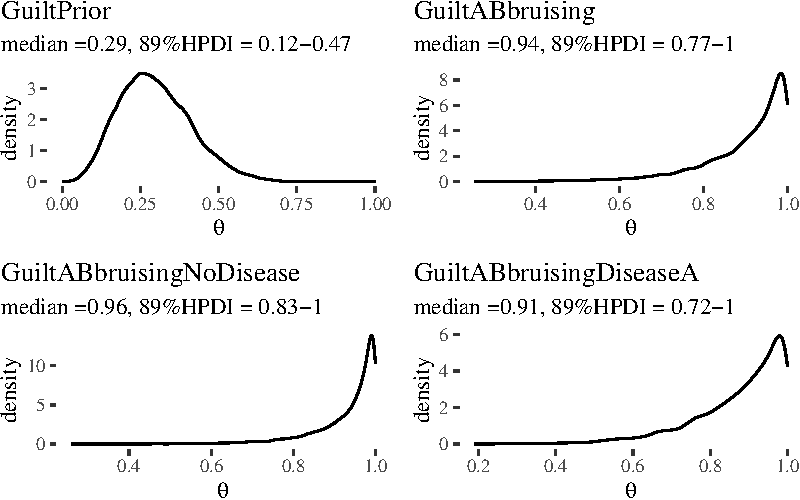
\includegraphics[width=0.9\textwidth,height=\textheight]{imp_philosophical_backup_files/figure-pdf/fig-scwithhop2-1.pdf}

}

\caption{\label{fig-scwithhop2}Impact of incoming evidence in the Sally
Clark case.}

\end{figure}

One question that arises is how this approach relates to the standard
method of using likelihood ratios to report the value of the evidence.
On this approach, the conditional probabilities that are used in the
likelihood ratio calculations are estimated and come in a package with
an uncertainty about them. Accordingly, these uncertainties propagate:
to estimate the likelihood ratio while keeping track of the uncertainty
involved, we can sample probabilities from the selected distributions
appropriate for the conditional probabilities needed for the
calculations, then divide the corresponding samples, obtaining a sample
of likelihood ratios, thus approximating the density capturing the
recommended uncertainty about the likelihood ratio. Uncertainty about
likelihood ratio is just propagated uncertainty about the involved
conditional probabilities. For instance, we can use this tool to gauge
our uncertainty about the likelihood ratios corresponding to the signs
of bruising in son A and the presence of the symptoms of a potentially
lethal disease in son A (Figure~\ref{fig-sclrs}).

\begin{figure}[H]

{\centering 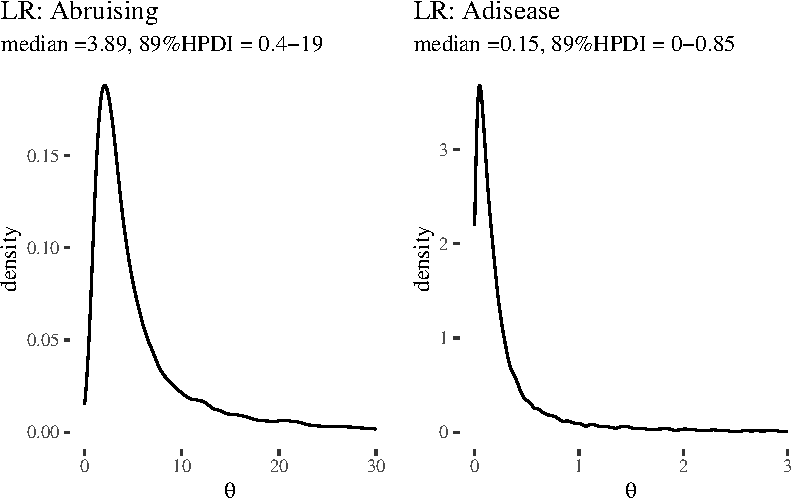
\includegraphics[width=0.9\textwidth,height=\textheight]{imp_philosophical_backup_files/figure-pdf/fig-sclrs-1.pdf}

}

\caption{\label{fig-sclrs}Likelihood ratios forbruising and signs of
disease in child A in the Sally Clark case.}

\end{figure}

\hypertarget{discussion}{%
\section{Discussion}\label{discussion}}

Our approach does involve multiple parameters, uncertainty about them,
along with a dependency structure between random variables. So it is
only natural to ask whether what we propose is not just an old wolf in a
new sheep's clothing, as one might think that what looks like a DAG and
quacks like a DAG is always a hierarchical model. In this section we
briefly clarify what the answer to this question is.

First, we need some clarity on what a Bayesian hierarchical model is. In
the widest sense of the word, these are mathematical descriptions
involving multiple parameters such that credible values for some of them
meaningfully depend on the values of other parameters, and that
dependencies can be re-factored into a chain of dependencies. For
instance, think about a joint parameter space for two parameters
\(\theta\) and \(\omega\), where
\(p(\theta, \omega \vert D) \propto p(D \vert \theta, \omega)p(\theta, \omega)\).
If, further, some independence-motivated re-factoring of the right-hand
side---for instance as
\(p(D\vert \theta)p(\theta \omega)p(\omega)\)---is possible, we are
dealing with a hierarchical model in the wide sense of the word.

Such models usually come useful when we are dealing with clustered data,
such as a cohort study with repeated measures, or some natural groupings
at different levels of analysis. Then, lower-level parameters are
treated as i.i.d. and share the same parameter distribution
characterized by some hyper-parameters in turn characterized by a prior
distribution. As a simple example consider a scenario in which we are
dealing with multiple coins created by one mint---each coin has its own
bias \(\theta_i\), but also there is some commonality as to what these
biases are in this mint, represented by a higher-level parameter
\(\theta\). Continuing the example, assume
\(\theta_i \sim \mathsf{Beta}(a, b)\) and
\(y_{i\vert s} \sim \mathsf{Bern}(\theta_s)\), where the former
distribution can be re-parametrized as
\(\mathsf{Beta}(\omega(k-2)+1, (1-\omega)(k-2)+1)\). Let's keep \(k\)
fixed, \(\omega\) is our expected value of the \(\theta_i\) parameters,
with some dispersion around it determined by \(k\). Now, if we also are
uncertain about \(\omega\) and express our uncertainty about it in terms
a density \(p(\omega)\), we got ourselves a hierarchical model with
joint prior distribution over parameters
\(\prod p(\theta_i \vert \omega) p(\omega)\).

As another example, one can develop a multilevel regression model of the
distributions of the random levels in various counties, where both the
intercept and the slope vary with counties by taking\\
\(y_i\sim \mathsf{Norm}(\alpha_{\mbox{j[i]}}\, + \beta_{\mbox{j[i]}} x_i, \sigma^2_y )\),
where \(j\) is a county index,
\(\alpha_j \sim \mathsf{Norm}(\mu_\alpha,\sigma_\alpha^2 )\), and
\(\beta_j \sim \mathsf{No}rm(\mu_\beta,\sigma_\beta^2 )\). Then, running
the regression one estimates both the county-level coefficients, and the
higher-level parameters.

Our approach is similar to the standard hierarchical models in the most
general sense:\\
there is a meaningful independence structure and distributions over
parameter values that we are working with. However, our approach is
unlike such models in a few respects. For one, we are not dealing with
clustered data, and the random variables are mostly propositions and
their truth values. Given a hypothesis \(H\) and an item of evidence
\(E\) for it, there seems to be no interesting conceptualization on
which the underlying data would be clustered. For example, considering
stains at a crime scene as a subgroup of crimes being committed doesn't
make logical sense. Yes, there is dependency between these phenomena,
but describing it as clustering would be at least misleading. Second,
the dependencies proceed through the values of the random variables
which are \textbf{not} parameters, but rather truth-values, and require
also conditional uncertainties regarding the dependencies between these
truth-values.

Again, continuing the hypothesis-evidence example, we have
\(H \sim \mathsf{Bern}(p_h)\), \(p_h \sim \mathsf{Beta}(a_h, b_h)\), and
\(E\sim \mathsf{Bern}(p_e)\). But then we also have the beta
distributions for the probability of the evidence conditional on the
actual values of the random variables---the truth-values---thus
\(p_e \vert H = 1 \sim beta(a_{+}, b_{+} )\) and
\(p_e \vert H = 0 \sim \mathsf{Beta}(a_{-}, b_{-})\). But the
re-factoring in terms of the actual values of the random variables
(which just happen to resemble probabilities because they are truth
values) makes it quite specific, at the same time allowing for the
computational use of a probabilistic program. Finally, the reasoning we
describe is not a regression the way it is normally performed: the
learning task is delegated to the bottom level of whatever happens to
the Bayesian networks once updated with evidence. We would prefer to
reserve the term \emph{hierarchical model} for a class of models dealing
with interesting cluster structures in the data. A more fitting term for
the representation tool we propose should be used here is
\emph{probabilistic programs}. We do not claim any originality in
devising this tool: it's an already existing tool. What we argue for,
though, is its ability for being usefully deployed in the context of
forensic evidence evaluation and integration with other assumptions and
hypotheses.

Perhaps, you might dislike the idea of going higher-order for
theoretical reasons. One might be that you don't like the complexity.
This seems to be the line taken by Bradley, who refuses to go
higher-order for the following reason:

\begin{quote}
Why is sets of probabilities the right level to stop the regress at? Why not sets of sets? Why not second-order 
probabilities? Why not single probability functions? This is something of a pragmatic choice. The further we 
allow this regress to continue, the harder it is to deal with these belief representing objects. So let's not
 go further than we need. 131-132\end{quote}

We have argued extensively, that given the difficulties of both PP and
IP and how the current approach handles it, we are not going further
than we need in using higher-order probabilities. We're going where we
should be. And the supposed pragmatic concerns that one might have are
unclear: parameter uncertainty, approximations and other computational
methods I have used in fact quite embedded in Bayesian statistical
practice and decent computational tools for the framework I propose are
available.\footnote{Also, you can insist that instead of
  going higher order we could just take our sample space to be the cartesian product of the original sample
   space and parameter space, or use parameters having certain values as potential states of a bayesian network. 
   If you prefer not to call such approaches first-order, I don't mind, as long as you effectively end up
    assigning probabilities to certain probabilities, the representation means I discussed in this paper
     should be in principle available to you.}

Another concern that you might have is that it is not clear what the
semantics of such an approach should look like. While a more elaborate
account is beyond the scope of this paper, the general gist of the
approach can be modeled by a slight modification of a framework of
probabilistic frames (Dorst, 2022b, 2022a). Start with a set of possible
worlds \(W\). Suppose you consider a class of probability distributions
\(D\), a finite list of atomic sentences \(q_1, \dots, q_2\)
corresponding to subsets of \(W\), and a selection of true probability
hypotheses \(C\) (think of the latter as omniscient distributions,
\(C\subseteq D\), but in principle this restriction can be dropped if
need be). Each possible world \(w\in W\) and a proposition
\(p\subseteq W\) come with their true probability distribution,
\(C_{w,p}\in D\) corresponding to the true probability of \(p\) in
\(w\), and the distribution that the expert assigns to \(p\) in \(w\),
\(P_{w,p}\in D\). Then, various propositions involving distributions can
be seen as sets of possible worlds, for instance, the proposition that
the expert assigns \(d\) to \(p\) is the set of worlds \(w\) such that
\(P_{w,p}=d\).\footnote{There is at least one important 
difference between this approach and that developed by Dorst. His  framework is untyped, which allows for 
an enlightening discussion of the principle of reflection and alternatives to it. In this paper I prefer 
to keep this complexity apart and use an explicitly typed set-up.}

\todo{Added this passage}

The reader might also be eager to point out that some of the techinques
we mentioned are already available to the impreciser. For instance, one
can use uniform sampling with Bayesian networks to approximate the
impreciser's epistemic commitments given their assumptions \todo{Cite 
\url{https://arxiv.org/abs/2302.09656}}. This doesn't mathematically
differ from relying on probabilistic programs with the restriction that
some variables corresponding to probabilities are sampled from
distributions that are uniform over a set of values determined by the
imprecisor's representor. However, this only shows that a computational
implementation of the impreciser's perspective is not out of
reach---which is to be expected. A critical survey of an approach along
these lines uses roughly this computational approach to argue that in
complex reasoning situations, if the imprecisor's stance is taken, `'the
imprecision of inferences increases rapidly as new premises are added to
an argument''.\todo{add ref to 
 \url{https://www.sciencedirect.com/science/article/pii/S0004370296000215}}
This is in line with our criticism.

\hypertarget{appendix-propriety}{%
\section*{Appendix: propriety}\label{appendix-propriety}}
\addcontentsline{toc}{section}{Appendix: propriety}

\hypertarget{appendix-the-strict-propriety-of-mathcali_dkl2}{%
\section*{\texorpdfstring{Appendix: the strict propriety of
\(\mathcal{I}_{\dkl}^2\)}{Appendix: the strict propriety of \textbackslash mathcal\{I\}\_\{\textbackslash dkl\}\^{}2}}\label{appendix-the-strict-propriety-of-mathcali_dkl2}}
\addcontentsline{toc}{section}{Appendix: the strict propriety of
\(\mathcal{I}_{\dkl}^2\)}

Let us start with a definition.

\begin{definition}[concavity]

A function $f$ is convex over an interval $(a,b)$ just in case for all  $x_1, x_2\in (a,b)$ and 
$0 \leq \lambda \leq 1$ we have:
\begin{align*}
f(\lambda x_1 + (1-\lambda)x_2) \leq \lambda f(x_1) + (1-\lambda)f(x_2)
\end{align*}

\noindent A function $f$  is concave just in case:
\begin{align*}
f(\lambda x_1 + (1-\lambda)x_2) \geq \lambda f(x_1) + (1-\lambda)f(x_2)
\end{align*}
\noindent A function $f$  is strictly concave just in case the equality holds only if either $\lambda = 0$ or $\lambda = 1$.
\end{definition}

For us it is important that if a function is twice differentiable on an
interval, then it is (strictly) concave just in case its second
derivative is non-positive (negative). In particular, as
\((\log_2(x))'' = -\frac{1}{x^2 ln(2)}\), \(\log_2\) is strictly concave
over its
domain.\footnote{I line with the rest of the paper, we'll work with $\log$ base 2. We could equally well use any other basis.}

\begin{lemma}[Jensen's inequality]
If $f$ is concave, and $g$ is any function of a random variable, $\mathbb{E}(f(g(x))) \leq f(\mathbb{E}(g(x)))$. If $f$ is 
strictly concave, the equality holds only if $g(x) = \mathbb{E} g(x)$, that is, if $g(x)$ is constant everywhere.
\end{lemma}

\begin{proof}
For the base case consider a two-point mass probability function. Then,
\begin{align*}
p_1f(g(x_1))+ p_2f(g(x_2)) &\leq f(p_1g(x_1) + p_2g(x_2))
\end{align*}
\noindent follows directly from the definition of concativity, if we take $\lambda = p_1$, $(1-\lambda)=p_2$,
 and substitute $g(x_1)$ and $g(x+2)$ for $x_1$ and $x_2$.



Now, suppose that  $ p_1f(g(x_1))+ p_2f(g(x_2)) = f(p_1g(x_1) + p_2g(x_2))$ and that   $f$ is strictly concave.
 That means either $(p_1 = 1\wedge p_2 = 0)$, or $(p_1 = 0 \wedge p_2 =1)$. Then either $x$ always takes
  value $x_1$, in the former case, or always takes value $x_2$, in the latter
   case. $\mathbb{E} g (x) =  p_1 g(x_1) + p_2 g(x_2)$, which equals  $g(x_1)$ in the former case and $g(x_2)$ in the latter.


Now suppose Jensen's inequality and the consequence of strict contativity) holds for $k-1$ mass points. 
Write $p_i' = \frac{p_i}{1-p_k}$ for $i = 1, 2, \dots, k-1$. We now reason:
\begin{align*}
\sum_{i=1}^k p_i f(g(x_i)) & =
 p_kf(g(x_k)) + (1-p_k)\sum_{i =1}^{k-1}p_i'f(g(x_i)) &\\
 & \leq p_k f(g(x_k)) + (1-p_k)f\left( \sum_{i = 1}^{k=i}p_i' g(x_i) \right) & \mbox{\footnotesize by 
 the induction hypothesis}\\ &\leq f\left( p_k(g(x_k)) + (1-p_k)\sum_{i = 1}^{k-1} p_i' g(x_i)\right) & 
 \mbox{\footnotesize by the base case} \\
 & = f \left( \sum_{i}^k p_i g(x_i)\right)
 \end{align*}

Notice also that at the induction hypothesis application stage we know that the equality holds only if 
$p_k =1 \vee p+k = 0$. In the former case $g(x)$ always takes value $x_k = \mathbb{E} g(x)$. In the latter case,
 $p_k$ can be safely ignored and $\sum_{i=1}^{k}p_ig(x_i) = \sum_{i=1}^{k-1}p'g(x_i)$ and by the induction 
 hypothesis we already know that $\mathbb{E} g(x) = g(x)$.


\end{proof}

In particular, the claim holds if we take \(g(x)\) to be
\(\frac{q(x)}{p(x)}\) (were both \(p\) and \(q\) are probability mass
functions), and \(f\) to be \(\log_2\). Then, given that \(A\) is the
support set of \(p\), we have: \begin{align*}
\sum_{x\in A}p(x) \log_2 \frac{q(x)}{p(x)} & \leq \log_2 \sum_{x\in A}p(x)\frac{q(x)}{p(x)}
\end{align*}

\noindent Moreover, the equality holds only if \(\frac{q(x)}{p(x)}\) is
constant, that is, only if \(p\) and \(q\) are the same pmfs. Let's use
this in the proof of the following lemma.

\begin{lemma}[Information inequality] For two probability mass functions $p, q$, $\dkl(p,q)\geq 0$ with 
equality iff $p=q$.
\end{lemma}

\begin{proof}
Let $A$ be the support set of $p$, and let $q$ be a probability mass function whose support is $B$.
\begin{align*}
- \dkl(p,q) & = - \sum_{x\in A}p(x) \log_2 \frac{p(x)}{q(x)}& \mbox{\footnotesize (by definition)} \\
&  =  \sum_{x\in A}p(x)  - \left(\log_2 p(x) - \log_2 q(x)\right)& \\
&  =  \sum_{x\in A}p(x)   \left(\log_2 q(x) - \log_2 p(x)\right)& \\
& =  \sum_{x\in A} p(x) \log_2 \frac{q(x)}{p(x)}& \\
& \leq \log_2 \sum_{x\in A} p(x)\frac{q(x)}{p(x)} & \mbox{\footnotesize by Jensen's inequality}\\
& \mbox{(and the equality holds only if $p = q$)}\\
& = \log_2 \sum_{x\in A} q(x)  & \\
& \leq \log_2 \sum_{x\in B} q(x) & \\
& = log (1)  = 0 &\\
\end{align*}
\end{proof}

Observe now that \(\dkl\) can be decomposed in terms of cross-entropy
and entropy.

\begin{lemma}[decomposition] $\dkl = H(p,q) - H(p)$. \end{lemma}

\begin{proof}
\begin{align*}
\dkl (p, q) & = \sum_{p_{i}} \left( \log_2 p_i - \log_2 q_i \right) \\
& =   - \sum_{p_{i}}\left( \log_2 q_{i} - \log_2 p_{i} \right) \\
& = - \sum_{p_{i}} \log_{2} q_{i} - \sum_{p_{i}} - \log_{2} p_{i}   \\
& -  \underbrace{- \sum_{p_{i}} \log_2 q_{i}}_{H(p,q)}    - \underbrace{- \sum_{p_i}  \log_2 p_{i}}_{H(p)}
\end{align*}
\end{proof}

With information inequality this easily entails Gibbs' inequality:

\begin{lemma}[Gibbs' inequality] $H(p,q) \geq H(p)$ with identity only if $p = q$.
\end{lemma}

Now we are done with our theoretical set-up. Here is how it entails the
propriety of \(\mathcal{I}_{\dkl}^2\). First, let's systematize the
notation. Consider a discretization of the parameter space \([0,1]\)
into \(n\) equally spaced values \(\theta_1, \dots, \theta_n\). For each
\(i\) the ``true'\,' second-order distribution if the true parameter
indeed is \(\theta_i\)---we'll call it the indicator of \(\theta_i\)---
is defined by \begin{align*}
Ind^k(\theta_i) & = \begin{cases} 1 & \mbox{if } \theta_i = \theta_k\\
                        0 & \mbox{otherwise}  \end{cases}
\end{align*} \noindent I will write \(Ind^k_i\) instead of
\(Ind^k(\theta_i)\).

Now consider a probability distribution \(p\) over this parameter space,
assigning probabilities \(p_1, \dots, p_n\) to
\(\theta_1, \dots, \theta_n\) respectively. It is to be evaluated in
terms of inaccuracy from the perspective of a given `true' value
\(\theta_k\). The inaccuracy of \(p\) if \(\theta_k\) is the `true'
value, is the divergence between \(IndI^k\) and \(p\).

\begin{align*}
\mathcal{I}_{\dkl}^2(p, \theta_k) & = \dkl(Ind^k,p) \\
& = \sum_{i=1}^n Ind^k_i \left( \log_2 Ind^k_i - \log_2 p_i \right)
\end{align*} Note now that for \(j \neq k\) we have \$Ind\^{}k\_j = 0 \$
and so \(Ind^k_j \left( \log_2 Ind^k_j - \log_2 p_j \right)=0\).
Therefore we continue: \begin{align*}
& = Ind^k_k \left( \log_2 Ind^k_k - \log_2 p_k \right)
\end{align*} Further, \(Ind^k_k= 1\) and therefore
\(\log_2 Ind^k_k =0\), so we simplify: \begin{align*}
& =  - \log_2 p_k
\end{align*}

\noindent Now, let's think about expected values. First, what the
inaccuracy of \(p\) as expected by \(p\), \(EI(p,p)\)?

\begin{align*}
EI(p,p) & = \sum_{i =1}^n p_i \mathcal{I}_{\dkl}^2(p, \theta_k) \\
& = \sum_{i =1}^n  p_i - \log_2 p_k \\
& = - \sum_{i =1}^n  p_i  \log_2 p_k = H(p)
\end{align*}

\noindent Analogously, the inaccuracy of \(q\) as expected from the
perspective of \(p\) is:

\begin{align*}
EI(p, q) & =   \sum_{i =1}^n p_i \left( - \log_2 q_i\right)\\
& = -  \sum_{i =1}^n p_i  \log_2 q_i) = H(p,q)
\end{align*}

But that means, by Gibbs' inequality, that \(EI(p,q) \geq EI(p,p)\)
unless \(p=q\), which completes the proof.

\hypertarget{references}{%
\section*{References}\label{references}}
\addcontentsline{toc}{section}{References}

\hypertarget{refs}{}
\begin{CSLReferences}{1}{0}
\leavevmode\vadjust pre{\hypertarget{ref-Bingham2021PPwithoutTears}{}}%
Bingham, E., Koppel, J., Lew, A., Ness, R., Tavares, Z., Witty, S., \&
Zucker, J. (2021). Causal probabilistic programming without tears.
\emph{Proceedings of the Third Conference on Probabilistic Programming}.

\leavevmode\vadjust pre{\hypertarget{ref-bradley2012scientific}{}}%
Bradley, S. (2012). \emph{Scientific uncertainty and decision making}
(PhD thesis). London School of Economics; Political Science (University
of London).

\leavevmode\vadjust pre{\hypertarget{ref-bradley2019imprecise}{}}%
Bradley, S. (2019). {Imprecise Probabilities}. In E. N. Zalta (Ed.),
\emph{The {Stanford} encyclopedia of philosophy} ({S}pring 2019).
\url{https://plato.stanford.edu/archives/spr2019/entries/imprecise-probabilities/};
Metaphysics Research Lab, Stanford University.

\leavevmode\vadjust pre{\hypertarget{ref-CampbellMoore2020accuracy}{}}%
Campbell-Moore, C. (2020). \emph{Accuracy and imprecise probabilities}.

\leavevmode\vadjust pre{\hypertarget{ref-Carr2020impreciseEvidence}{}}%
Carr, J. R. (2020). Imprecise evidence without imprecise credences.
\emph{Philosophical Studies}, \emph{177}(9), 2735--2758.
\url{https://doi.org/10.1007/s11098-019-01336-7}

\leavevmode\vadjust pre{\hypertarget{ref-deadman1984fiber2}{}}%
Deadman, H. A. (1984a). Fiber evidence and the wayne williams trial
(conclusion). \emph{FBI L. Enforcement Bull.}, \emph{53}, 10--19.

\leavevmode\vadjust pre{\hypertarget{ref-deadman1984fiber1}{}}%
Deadman, H. A. (1984b). Fiber evidence and the wayne williams trial
(part i). \emph{FBI L. Enforcement Bull.}, \emph{53}, 12--20.

\leavevmode\vadjust pre{\hypertarget{ref-Dorst2022evidence}{}}%
Dorst, K. (2022a). Higher-order evidence. In M. Lasonen-Aarnio \& C.
Littlejohn (Eds.), \emph{The routledge handbook for the philosophy of
evidence}. Routledge.

\leavevmode\vadjust pre{\hypertarget{ref-Dorst2022higher-order}{}}%
Dorst, K. (2022b). Higher-order uncertainty. In M. Skipper \& A. S.
Petersen (Eds.), \emph{Higher-order evidence: New essays}.

\leavevmode\vadjust pre{\hypertarget{ref-Lee2017impreciseEpistemology}{}}%
Elkin, L. (2017). \emph{Imprecise probability in epistemology} (PhD
thesis). Ludwig-Maximilians-Universit{ä}t;
Ludwig-Maximilians-Universität München.

\leavevmode\vadjust pre{\hypertarget{ref-Fenton2018Risk}{}}%
Fenton, N., \& Neil, M. (2018). \emph{Risk assessment and decision
analysis with bayesian networks}. Chapman; Hall.

\leavevmode\vadjust pre{\hypertarget{ref-VanFraassen2006vague}{}}%
Fraassen, B. C. V. (2006). Vague expectation value loss.
\emph{Philosophical Studies}, \emph{127}(3), 483--491.
\url{https://doi.org/10.1007/s11098-004-7821-2}

\leavevmode\vadjust pre{\hypertarget{ref-Gardenfors1982unreliable}{}}%
Gärdenfors, P., \& Sahlin, N.-E. (1982). Unreliable probabilities, risk
taking, and decision making. \emph{Synthese}, \emph{53}(3), 361--386.
\url{https://doi.org/10.1007/bf00486156}

\leavevmode\vadjust pre{\hypertarget{ref-GneitRafter2007}{}}%
Gneiting, T., \& Raftery, A. E. (2007). Strictly proper scoring rules,
prediction, and estimation. \emph{Journal of the American Statistical
Association}, \emph{102}(477), 359--378.
\url{https://doi.org/10.1198/016214506000001437}

\leavevmode\vadjust pre{\hypertarget{ref-HersbachDecomp2000}{}}%
Hersbach, H. (2000). Decomposition of the continuous ranked probability
score for ensemble prediction systems. \emph{Weather and Forecasting},
\emph{15}(5), 559--570.
https://doi.org/\url{https://doi.org/10.1175/1520-0434(2000)015\%3C0559:DOTCRP\%3E2.0.CO;2}

\leavevmode\vadjust pre{\hypertarget{ref-joyce2005probabilities}{}}%
Joyce, J. (2005). How probabilities reflect evidence.
\emph{Philosophical Perspectives}, \emph{19}(1), 153--178.

\leavevmode\vadjust pre{\hypertarget{ref-Kaplan1968decision}{}}%
Kaplan, J. (1968). Decision theory and the fact-finding process.
\emph{Stanford Law Review}, \emph{20}(6), 1065--1092.

\leavevmode\vadjust pre{\hypertarget{ref-keynes1921treatise}{}}%
Keynes, J. M. (1921). \emph{A treatise on probability, 1921}. London:
Macmillan.

\leavevmode\vadjust pre{\hypertarget{ref-konek2013foundations}{}}%
Konek, J. (2013). \emph{New foundations for imprecise bayesianism} (PhD
thesis). University of Michigan.

\leavevmode\vadjust pre{\hypertarget{ref-kruschke2015doing}{}}%
Kruschke, J. (2015). \emph{Doing bayesian data analysis (second
edition)}. Boston: Academic Press.

\leavevmode\vadjust pre{\hypertarget{ref-Kyburg1961}{}}%
Kyburg, H. E. (1961). \emph{Probability and the logic of rational
belief}. Wesleyan University Press.

\leavevmode\vadjust pre{\hypertarget{ref-kyburg2001uncertain}{}}%
Kyburg Jr, H. E., \& Teng, C. M. (2001). \emph{Uncertain inference}.
Cambridge University Press.

\leavevmode\vadjust pre{\hypertarget{ref-Levi1974ideterminate}{}}%
Levi, I. (1974). On indeterminate probabilities. \emph{The Journal of
Philosophy}, \emph{71}(13), 391. \url{https://doi.org/10.2307/2025161}

\leavevmode\vadjust pre{\hypertarget{ref-Levi1980enterprise}{}}%
Levi, I. (1980). \emph{The enterprise of knowledge: An essay on
knowledge, credal probability, and chance}. MIT Press.

\leavevmode\vadjust pre{\hypertarget{ref-Mayo-Wilson2016scoring}{}}%
Mayo-Wilson, C., \& Wheeler, G. (2016). Scoring imprecise credences: A
mildly immodest proposal. \emph{Philosophy and Phenomenological
Research}, \emph{92}(1), 55--78.
\url{https://doi.org/10.1111/phpr.12256}

\leavevmode\vadjust pre{\hypertarget{ref-o2006uncertain}{}}%
O'Hagan, A., Buck, C. E., Daneshkhah, A., Eiser, J. R., Garthwaite, P.
H., Jenkinson, D. J., \ldots{} Rakow, T. (2006). \emph{Uncertain
judgements: Eliciting experts' probabilities}.

\leavevmode\vadjust pre{\hypertarget{ref-Pettigrew2012Epistemic-Utili}{}}%
Pettigrew, R. (2012). \emph{Epistemic utility and norms for credences}.

\leavevmode\vadjust pre{\hypertarget{ref-Rinard2013against}{}}%
Rinard, S. (2013). Against radical credal imprecision. \emph{Thought: A
Journal of Philosophy}, \emph{2}(1), 157--165.
\url{https://doi.org/10.1002/tht3.84}

\leavevmode\vadjust pre{\hypertarget{ref-Schoenfield2017accuracy}{}}%
Schoenfield, M. (2017). The accuracy and rationality of imprecise
credences. \emph{Noûs}, \emph{51}(4), 667--685.
\url{https://doi.org/10.1111/nous.12105}

\leavevmode\vadjust pre{\hypertarget{ref-seidenfeld2012forecasting}{}}%
Seidenfeld, T., Schervish, M., \& Kadane, J. (2012). Forecasting with
imprecise probabilities. \emph{International Journal of Approximate
Reasoning}, \emph{53}, 1248--1261.
\url{https://doi.org/10.1016/j.ijar.2012.06.018}

\leavevmode\vadjust pre{\hypertarget{ref-Sturgeon2008grain}{}}%
Sturgeon, S. (2008). Reason and the grain of belief. \emph{No{û}s},
\emph{42}(1), 139--165. Retrieved from
\url{http://www.jstor.org/stable/25177157}

\leavevmode\vadjust pre{\hypertarget{ref-walley1991statistical}{}}%
Walley, P. (1991). \emph{Statistical reasoning with imprecise
probabilities}. Chapman; Hall London.

\end{CSLReferences}



\end{document}
